%%%%%%%%%%%%%%%%%%%%%%%%%%%%%%%%%%%%
\chapter{Introduction}
\label{chap:Introduction}
%%%%%%%%%%%%%%%%%%%%%%%%%%%%%%%%%%%%



\section{Background}
\label{background}
\epigraph{We are of course, supposing for the present that the questions are of the kind to which an answer `Yes' or `No' is appropriate, rather than questions such as `What do you think of Picasso?'\cite{TURING1950}}{\textit{Alan M. Turing
}}

\cite{sal2021, Raiyani2021, Helber2017, Mazzia2020, Baamonde2019}  
Image aesthetic assessment as a computational and machine learning task is important, challenging and fascinating. The application of aesthetics is wide, and encompasses areas such as cosmetics, calligraphy, and painting alongside beauty prediction of digital portraits\cite{Redi2015a} and facial beauty prediction\cite{Gray2010,Eisenthal2006a, Zhang2016}. Applications within the art domain include style recognition\cite{Cho2020, Fernando2021} and aesthetic visual quality of handwriting\cite{Sun2015}. All of these approaches require some form of digital imagery, and this thesis will focus on the Aesthetic Quality Assessment of digital images in the form of digital photographs. \par 

Within computer vision, there are sub-domains where aesthetics is a component such as Image Quality Assessment(IQA)\cite{Gu2020,Seshadrinathan2009,Sheikh2005,Ke2006,Chubarau2021,Reisenhofer2018} and Image Restoration, which have used metrics such as PSNR and SSIM. However, Image Aesthetic Quality Assessment(IAQA) treats aesthetic prediction as a target rather than focusing necessarily on individual image properties. Where IQA and image restoration have focused on restoring objective image distortions and are aimed at modelling or predicting a physical property such that it can be removed, IAQA focuses on predicting classes or aesthetics attributes.

\par
 
While aesthetic is often based on individual subjective perception, it is important to demarcate this from objective and empirical study within the field of machine learning and pattern recognition. Where the focus is on objective ground truth, whether by experts or aggregated scores, the computer vision task is to best predict ground truth. The perceptual element, alongside the potential for ambiguity and lack of consensus on concepts such 'beauty' and 'aesthetic appreciation'\cite{Datta2006}, add to the complexity and the challenge of IAQA\cite{Yang2019} as a machine learning problem. One aspect of this is that it includes human visual perception, which has been shown within psychological studies to be both contingent upon the target photograph's context\cite{Mullennix2020}, where the order in which images are viewed effects aesthetic perception, and to differ significantly between subjects\cite{Younes2016}. 

\newpage

IAQA's reliance upon high-level social concepts\cite{Datta2006} is however part of what makes the field so fascinating; with the potential to further insights into human visual attention, perception, and cognition\footnote{\textit{Vision} it might be argued it is a form of perception, property of cognition and intelligence\cite{russell2016artificial} . Pigeons for instance have been shown to be remarkable observers of pathology \cite{Levenson2015} when rewarded appropriately.
} and continue a valuable tradition of biologically inspired computing\cite{Hassabis2017} that began in the 1950s, in addition of course to IAQA's significant commercial and practical applications. 

\par 
Computer vision has made significant gains in tasks such as object recognition, classification, medical imaging\cite{Esteva2021}.  The problem of 'vision' is however far from solved; for example, semantic scene detection remains a challenging area of focus. This is complex in part because it requires consideration of whether image segmentation \textit{or} recognition comes first\cite{Kreiman2021} (a task that can also be a challenge for humans) (see figure \ref{fig:vase_face}). IAQA is one such challenging domain application.\par



\begin{figure}[h!]
    \centering
    \subfloat[Vase Face Figure Ground ambiguity f \cite{Hobbs1990,Eysenk2012}]{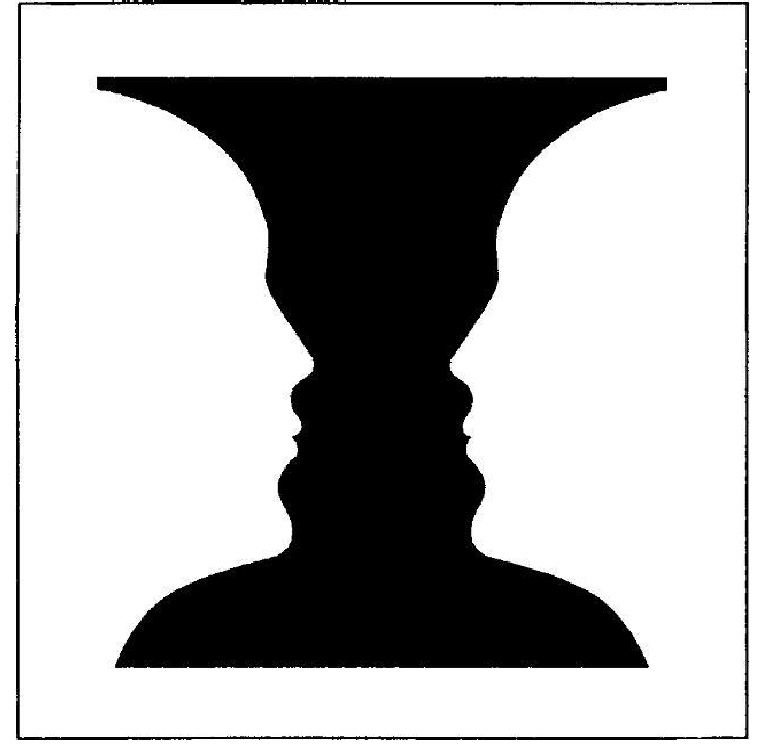
\includegraphics[height=0.2\textwidth]{figures/introduction/face-vase-face.png}}
    \subfloat[ An average face with a Phi mask not fitting the average face well \cite{Zhang2016}]{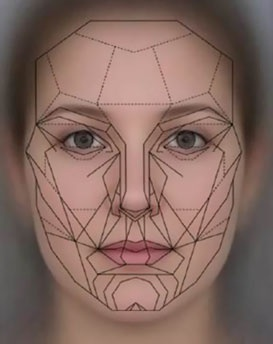
\includegraphics[height=0.2\textwidth]{figures/introduction/1492016_Book_ComputerModelsForFacialBeautyA.pdf1.jpeg}}
    \caption{Examples of Ambiguity for Machines and Humans}
    \label{fig:vase_face}
\end{figure}

\par

Traditional approaches to IQA have aimed at measuring image distortion by degrees\cite{gonzalez2008digital} within the wider field of digital image restoration. IQA's focus on modelling the non-commutative and non associative process of restoring digital image distortions caused by the corpuscular nature of light such as diffraction, refraction or image sensor noise caused during the capture of digital images in low light conditions.\cite{szeliski2011computer,gonzalez2008digital} have informed approaches to early approaches IAQA. In both IAQA and IQA, traditional computer vision has been superseded by Machine Learning(ML) in many areas, using techniques such as Deep Learning using convolutional neural networks (CNNs) which have been successfully employed since first used for character recognition\cite{LeCun1989,LeCun1998}.  \par
This thesis will examine how these more recent techniques have been applied to challenging domain application of IAQA, and seek to improve and  demonstrate effectiveness of different deep learning approaches within IAQA.

\newpage


\subsection{The Application Domain}

The Oxford English Dictionary(OED) defined 'aesthetics' as 'Of or relating to the perception, appreciation, or criticism of that which is beautiful'\cite{OED2021}. Aesthetics more widely includes appreciation of all senses, including touch and olfactory sensation\cite{Hayes2015}, and further cognitive activities such as mathematical problem solving which have an element of reward or pleasure, where we might consider a solution `elegant' or `beautiful'\cite{Rolls2014}. Aesthetics, therefore, can be considered a broad application domain that requires narrowing.  

\par

 Attempts to study aesthetics have been made within psychology (imperial aesthetics)\cite{Greb2017}, art criticism, philosophy, and as the subject of enquiry within the field of computer vision. IAQA, therefore, is a subset at the intersection of computer vision, aesthetics and image processing, focusing on digital photographic images. This might be considered a sub-domain within the wider field of visual aesthetics, where quality estimation or ranking is involved, and includes painting, calligraphy, cartoon imagery and sculptures. This section will provide a high-level overview of these interrelated fields and provide the framework for formulation IAQA as a computer vision problem. 

\subsection{Aesthetics Philosophy}

Philosophy gives the the earliest examples of formal enquiry into aesthetics by Plato\cite{Plochmann1976} (230-bc) and (1790)  in the west by E. Kant and E. Burke \cite{Kant1892kant, Burke1773philosophical}. This enquiry has continued into the 20th century with philosophers such as L. Wittgenstein\cite{Wittgenstien1967}, who, in making general observations on aesthetic, remarks that enumerable facial expressions can be highlighted by only subtle changes in four strokes (figure \ref{fig:faces})  contrasting it with figure \ref{fig:squiggle}. Wittgenstein remarks that such squiggles drawn one after the other would be indistinguishable; a humorous, insightful remark that demonstrates clearly how aesthetic consideration is both highly nuanced and complex. One might ask here if this is the case for machines? 
\begin{figure}[H]
    \centering
    \begin{subfigure}[b]{0.3\textwidth}
    \centering
    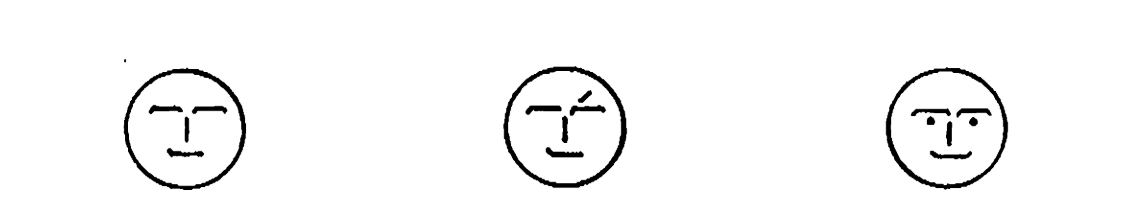
\includegraphics[width=\textwidth]{figures/introduction/faces.png}
    \caption{Faces}
    \label{fig:faces}
    \end{subfigure}
    \begin{subfigure}[b]{0.3\textwidth}
    \centering
    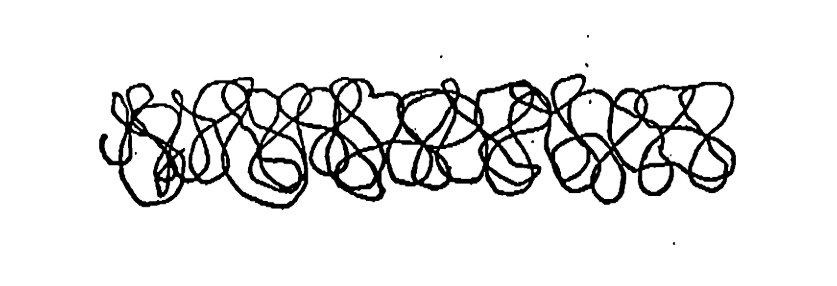
\includegraphics[width=\textwidth]{figures/introduction/squiggle_s.png}
    \caption{Squiggle S}
    \label{fig:squiggle}
    \end{subfigure}
    \caption{Left Faces, Right 'Squiggle S' \cite{Wittgenstien1967} }
    \label{fig:Witgenstein}
\end{figure}


\subsection{Empirical Aesthetics}

This domain covers a field of study within psychology and neuroscience where perception is studied using technologies such as eye tracking\cite{Younes2016} and leveraging environmental controls in experiments where subjects rank images. There is some overlap within the field of IAQA and its dataset, such as the Waterloo IAA\cite{Liu2017a}, where IAQA has used techniques normally applied within psychological experiments\footnote{A frequent critique of many IAQA datasets lack of control of ground truth data generation.}. 

\par

    %%%%%%
 %%%%%%%%%%%%%
   % %  % % 
       %    $$
     %%%%%

\begin{figure}[htp!]
\centering
\subfloat[Curve 2D Shape & Line]{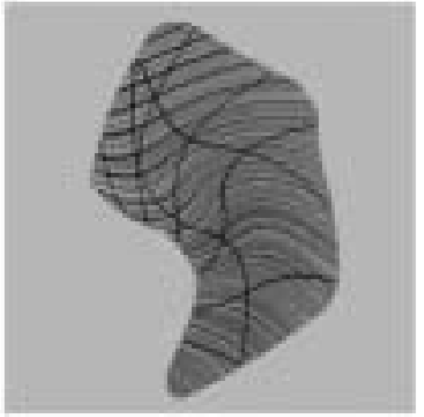
\includegraphics[width=0.15\textwidth]{figures/introduction/imperical aesthetics/curve.png}}
\subfloat[Non Curve 2D Shape & Line]{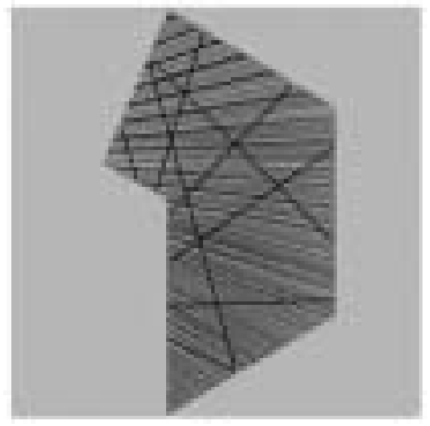
\includegraphics[width=0.15\textwidth]{figures/introduction/imperical aesthetics/non_curve.png}}
\subfloat[Curve Couch Design]{
  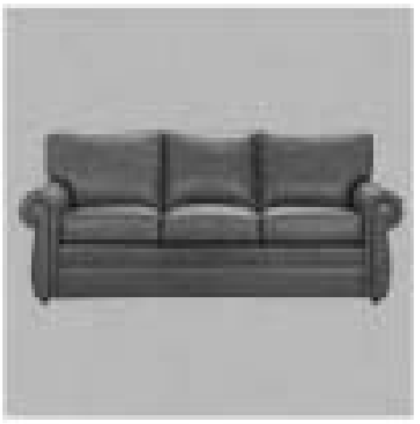
\includegraphics[width=0.15\textwidth]{figures/introduction/imperical aesthetics/curve_2.png}
}
\subfloat[Non-Curved Couch Design]{
  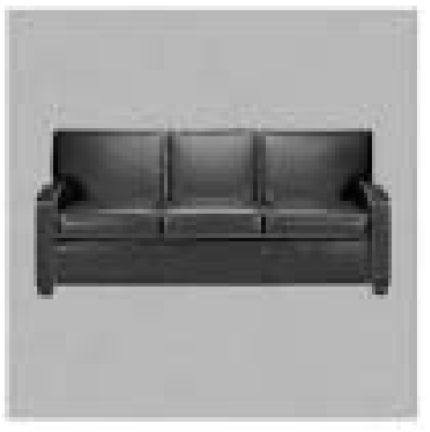
\includegraphics[width=0.15\textwidth]{figures/introduction/imperical aesthetics/non_curve_2.png}
 
}
\caption{Examples of Visual preference (a)(c) vs less pleasing (b)(d) \cite{Bar2006}}
\label{fig:curve}
\end{figure}

This is a relevant field, as it has provided  controls such as screen calibration, image display, subject demographic, and randomization of stimuli\cite{Leder2019,Mullennix2013, Rolls2014}. Empirical aesthetics also provides insight into areas such as visual symmetry, which are known to have also been a subject of computer vision\cite{Elawady2017,Gray2010}, and an understanding of how viewers might rank an image. 
\begin{figure}[H]
\centering
\subfloat[Random Image]{
  
\includegraphics[height=0.15\textwidth]{figures/introduction/imperical aesthetics/random_1.png}
  \label{fig:non_symetry}}
\subfloat[Symmetrical Image]{
  
\includegraphics[height=0.15\textwidth]{figures/introduction/imperical aesthetics/symetry.png}
  \label{fig:symetry_reflect}}
\subfloat[Rotational Symmetry Image]{
  
\includegraphics[height=0.15\textwidth]{figures/introduction/imperical aesthetics/rotational_symetry.png}
  \label{fig:symetry_rotation}}
\caption{Examples of images used in psychological experiments showing visual preference for symmetry and complexity      \cite{Bertamini2013}}
\label{fig:symetry}
\end{figure}


These studies have shown experimentally both that formal rules such as the 'golden ratio' and 'averageness' in facial portraits (figure \ref{fig:means}), symmetry (figure \ref{fig:symetry}), complexity\cite{Bertamini2013}, and curve (figure \ref{fig:curve}) are attributes that are associated with aesthetically pleasing design and images (figure \ref{fig:means}).

\begin{figure}[ht!]
    \centering
    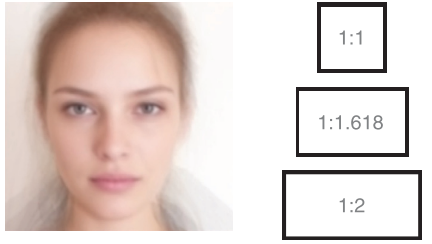
\includegraphics[width=0.3\textwidth]{figures/introduction/imperical aesthetics/means.png}
    \caption{Average Composite Face (left) , Golden Ratio (Middle Right) \cite{Brielmann2018}}
    \label{fig:means}
\end{figure}

\par

However, this is far from the whole `picture' and it has been shown both in computer vision \cite{Simond2015} and in imperial aesthetics publications alike that attributes such the golden ratio or rule of thirds in photography\cite{Green2012} and symmetry\cite{Leder2019} are not universal aesthetic attributes and depend on context - this underscores the complex nature inherent within the domain of aesthetics. 



\subsection{Art Aesthetics}

Art aesthetics and criticism include consideration of brush strokes and artist techniques, alongside the interpretation of images within cultural and critical studies that intersect with social sciences, literary criticisms and philosophy. \textit{Perspectives} within art aesthetics might consider or include \textit{Marxist, psychoanalytical, feminist (figure \ref{fig:femnist_art}) and queer (figure \ref{fig:mapplethorp}}). 

\par The tradition in the 20th century has been to apply intellectual theory that has also been applied to other art forms, such as film and literature, and is not limited to considerations of \textit{good} or \textit{bad} opinion but rather critical and conceptual analysis using vernacular such as `feminist aesthetics' or `feminist critique'\cite{Hein1990} of an artwork, item of popular culture or an image.

\par One fascinating feature of 20th century art is the inclusion of critical theory into the artwork aesthetics itself and `aesthetics' that are ironic or a pastiche of popular culture's aesthetics (figure \ref{fig:femnist_art} shows two renowned and striking examples of this). 
\begin{figure}[htp!]
\FloatBarrier
    \centering
    \subfloat[ (sic.) Untitled (Your Body is a Battleground)\footnote{Untitled is used ironically with inclusion of parenthetic title} \cite{Kruger1898}]{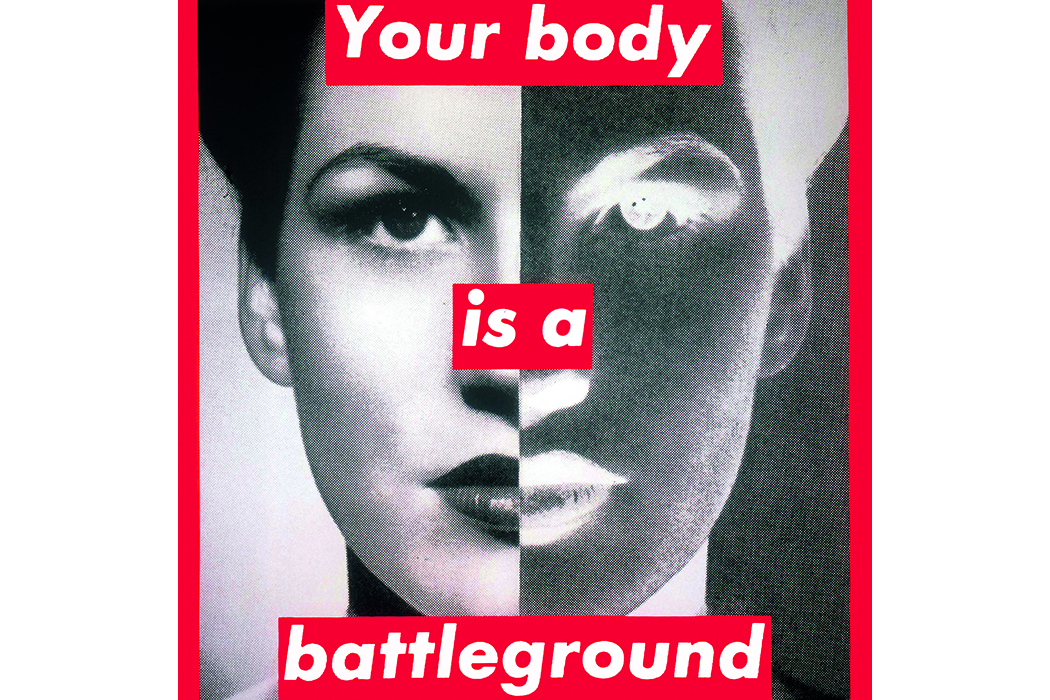
\includegraphics[height=0.2\textwidth]{figures/introduction/art aesthetics/Kruger_1050x700.jpg}}
    \hfill
    \subfloat[Do Women Have To Be Naked To Get Into the Met. Museum?\    \cite{TheGorillaGirls1989}]{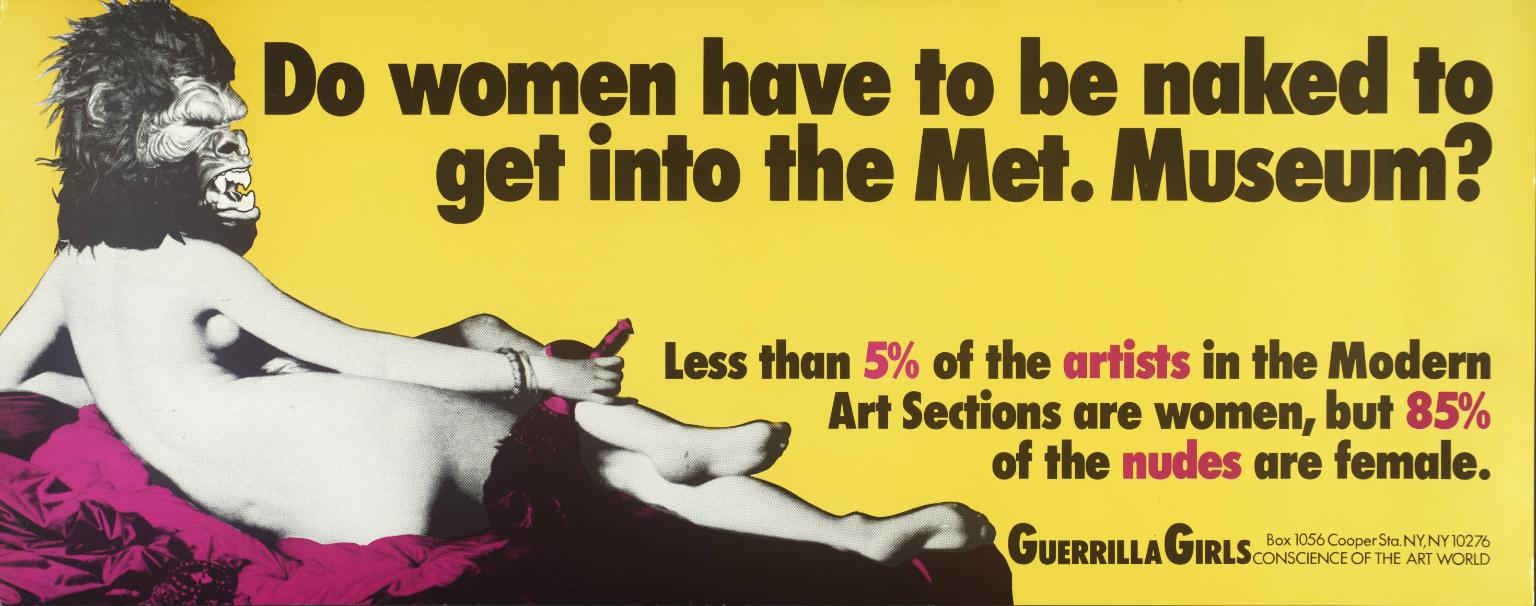
\includegraphics[height=0.2\textwidth]{figures/introduction/art aesthetics/gorrilla girls.jpg}}
    \caption{Examples of Late 20th century Feminist Artworks}
    \label{fig:femnist_art}
\end{figure}
\par Art aesthetics this are important and relevant in considering the possible applications of IAQA and given how different models that are trained apparently handle ambiguous examples and the potential to provide a `critical lens' on areas such as cultural, racial or gender bias that might be replicated by machines. One might ask here how computer vision might learn feminist aesthetics?

\par Much of the focus of IAQA has been on what might fall within extraction of features: formalist art aesthetics, such as lighting, perspective or particular aesthetic techniques such as chiaroscuro (using lighter or darker tonal values to make something appear three dimensional)\cite{Hobbs1990} shown in \ref{fig:chiaroscuro}. 
\par Another example of formalist aesthetics involves using attributes such as colour harmony - or using colours that are equidistant on a colour wheel (figure \ref{fig:colorwheel}) - which positions discrete colours according to position, following prismatic splitting (figure \ref{fig:newton}) (or electromagnetic spectrum) first theorized by Newton \textit{red, orange, yellow, green, blue, indigo, violet}.

\begin{figure}[ht!]
\centering
    \subfloat[Self Portrait by Artist Robert Mapplethorpe    \cite{Mapplthorpe1980}]{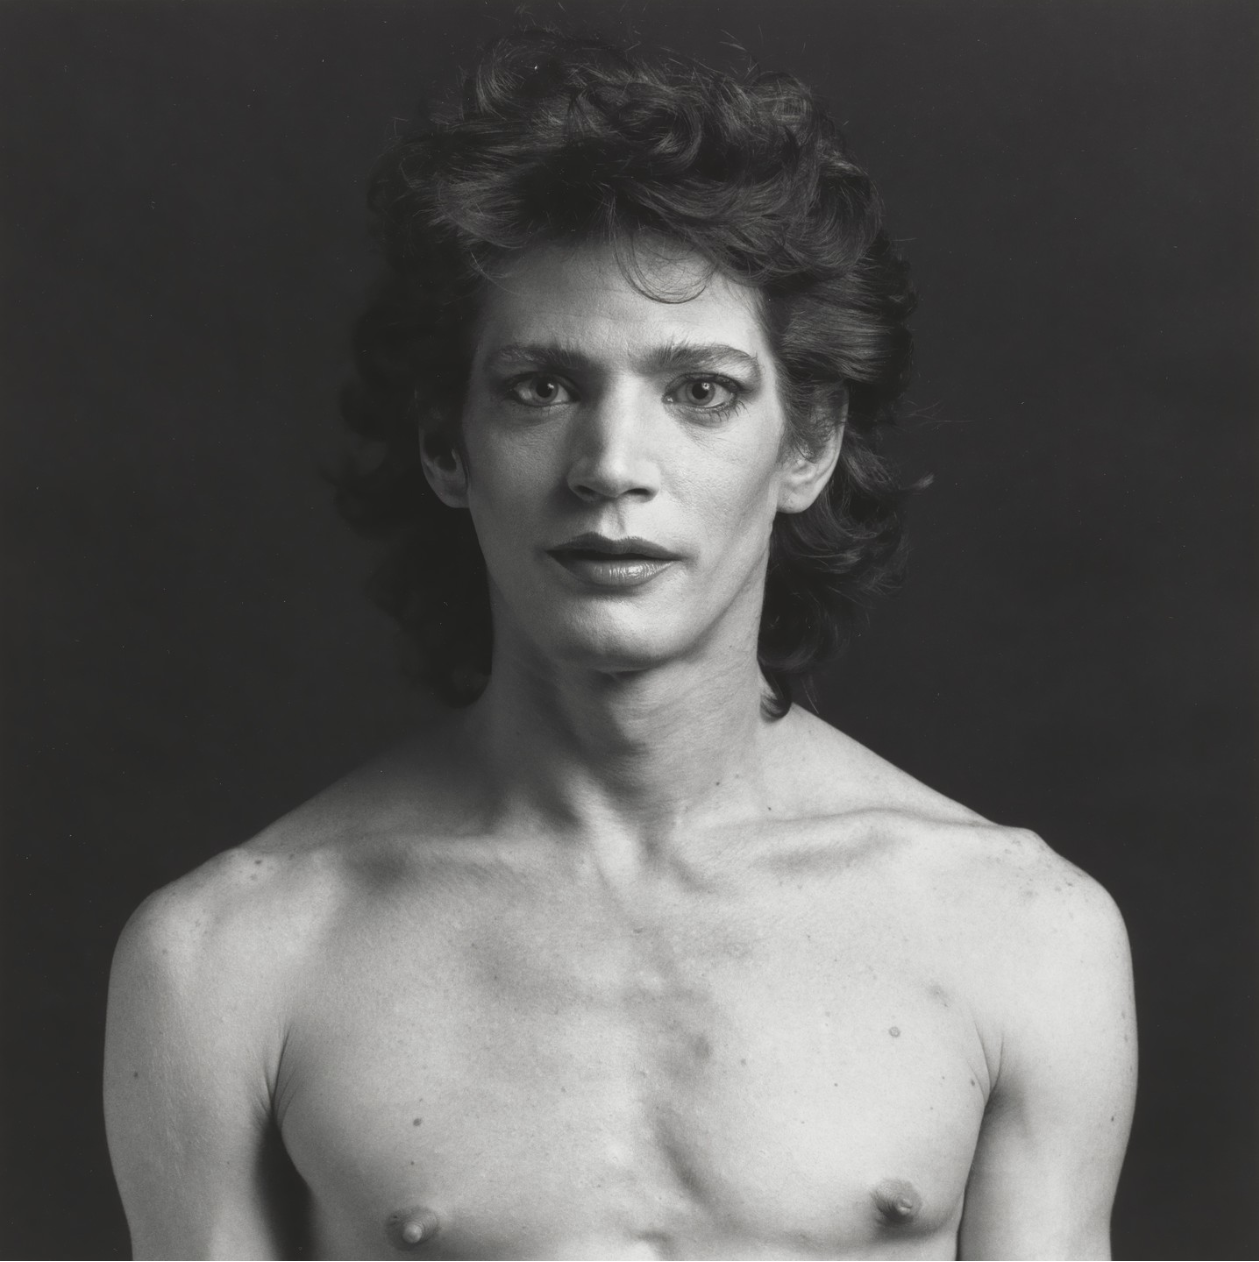
\includegraphics[width=0.2\textwidth]{figures/introduction/art aesthetics/mapplthorp.png}
    \label{fig:mapplethorp}}
    \hfill
    \subfloat[El Fabula(an Alegory) \cite{Domenikos1580}]{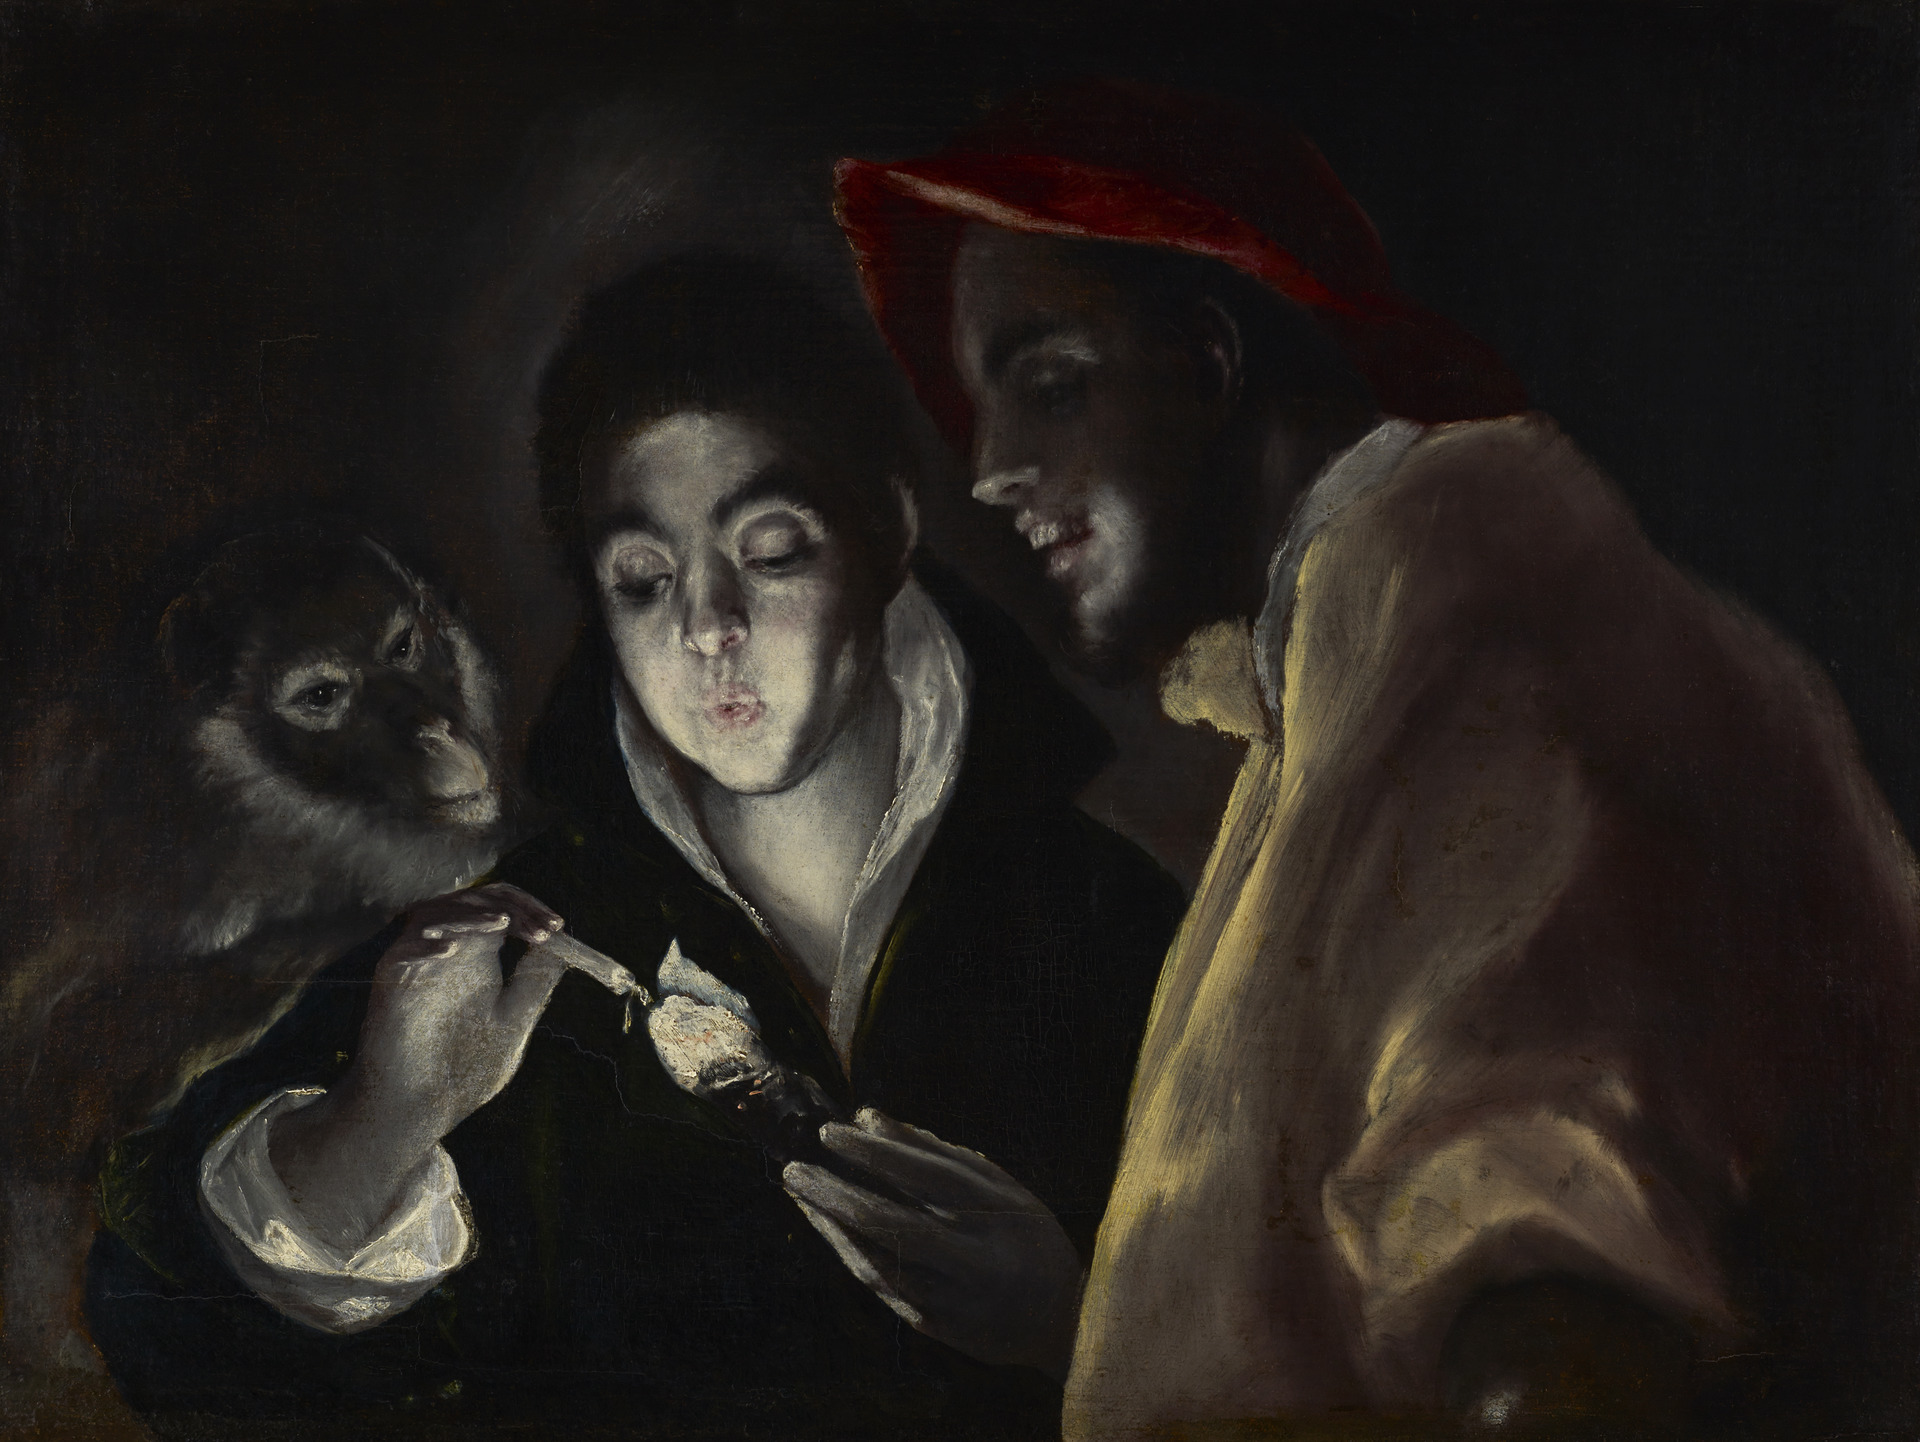
\includegraphics[width=0.2\textwidth]{figures/introduction/art aesthetics/an-allegory-f-bula.jpg}}
    \hfill
    \subfloat[Salome Receives the Head of John the Baptist   \cite{Caravaggio1609}]{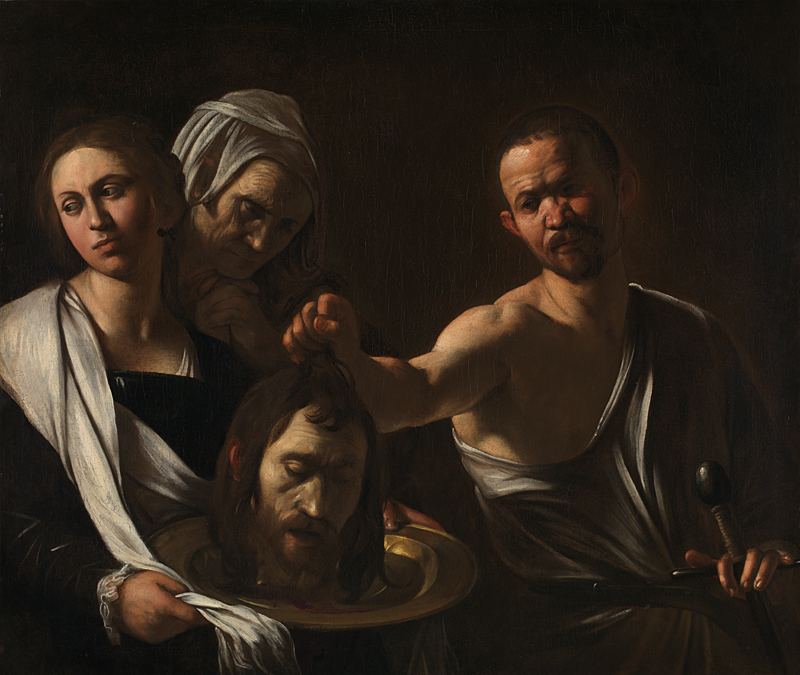
\includegraphics[width=0.2\textwidth]{figures/introduction/art aesthetics/carrivagio.jpg}}
    \caption{Chiaroscuro examples}
    \label{fig:chiaroscuro}
    \vfill 
    \subfloat[ Newton's Color Wheel Based on EMS (Prismatic Splitting)]{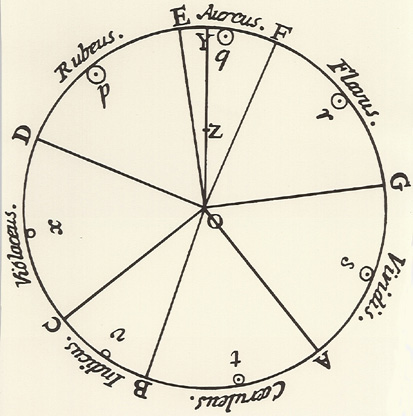
\includegraphics[width=0.2\textwidth]{figures/introduction/art aesthetics/Newton-Color-wheel.jpg}
    \label{fig:newton}}
    \hfill
    \subfloat[Primary and Secondary Hues in Pigments  \cite{Hobbs1990}]{
\includegraphics[width=0.2\textwidth]{figures/introduction/art aesthetics/chromatic_splitting.jpg}}
    \hfill
    \subfloat[ Aesthetics Color Wheel   \cite{Hobbs1990}]{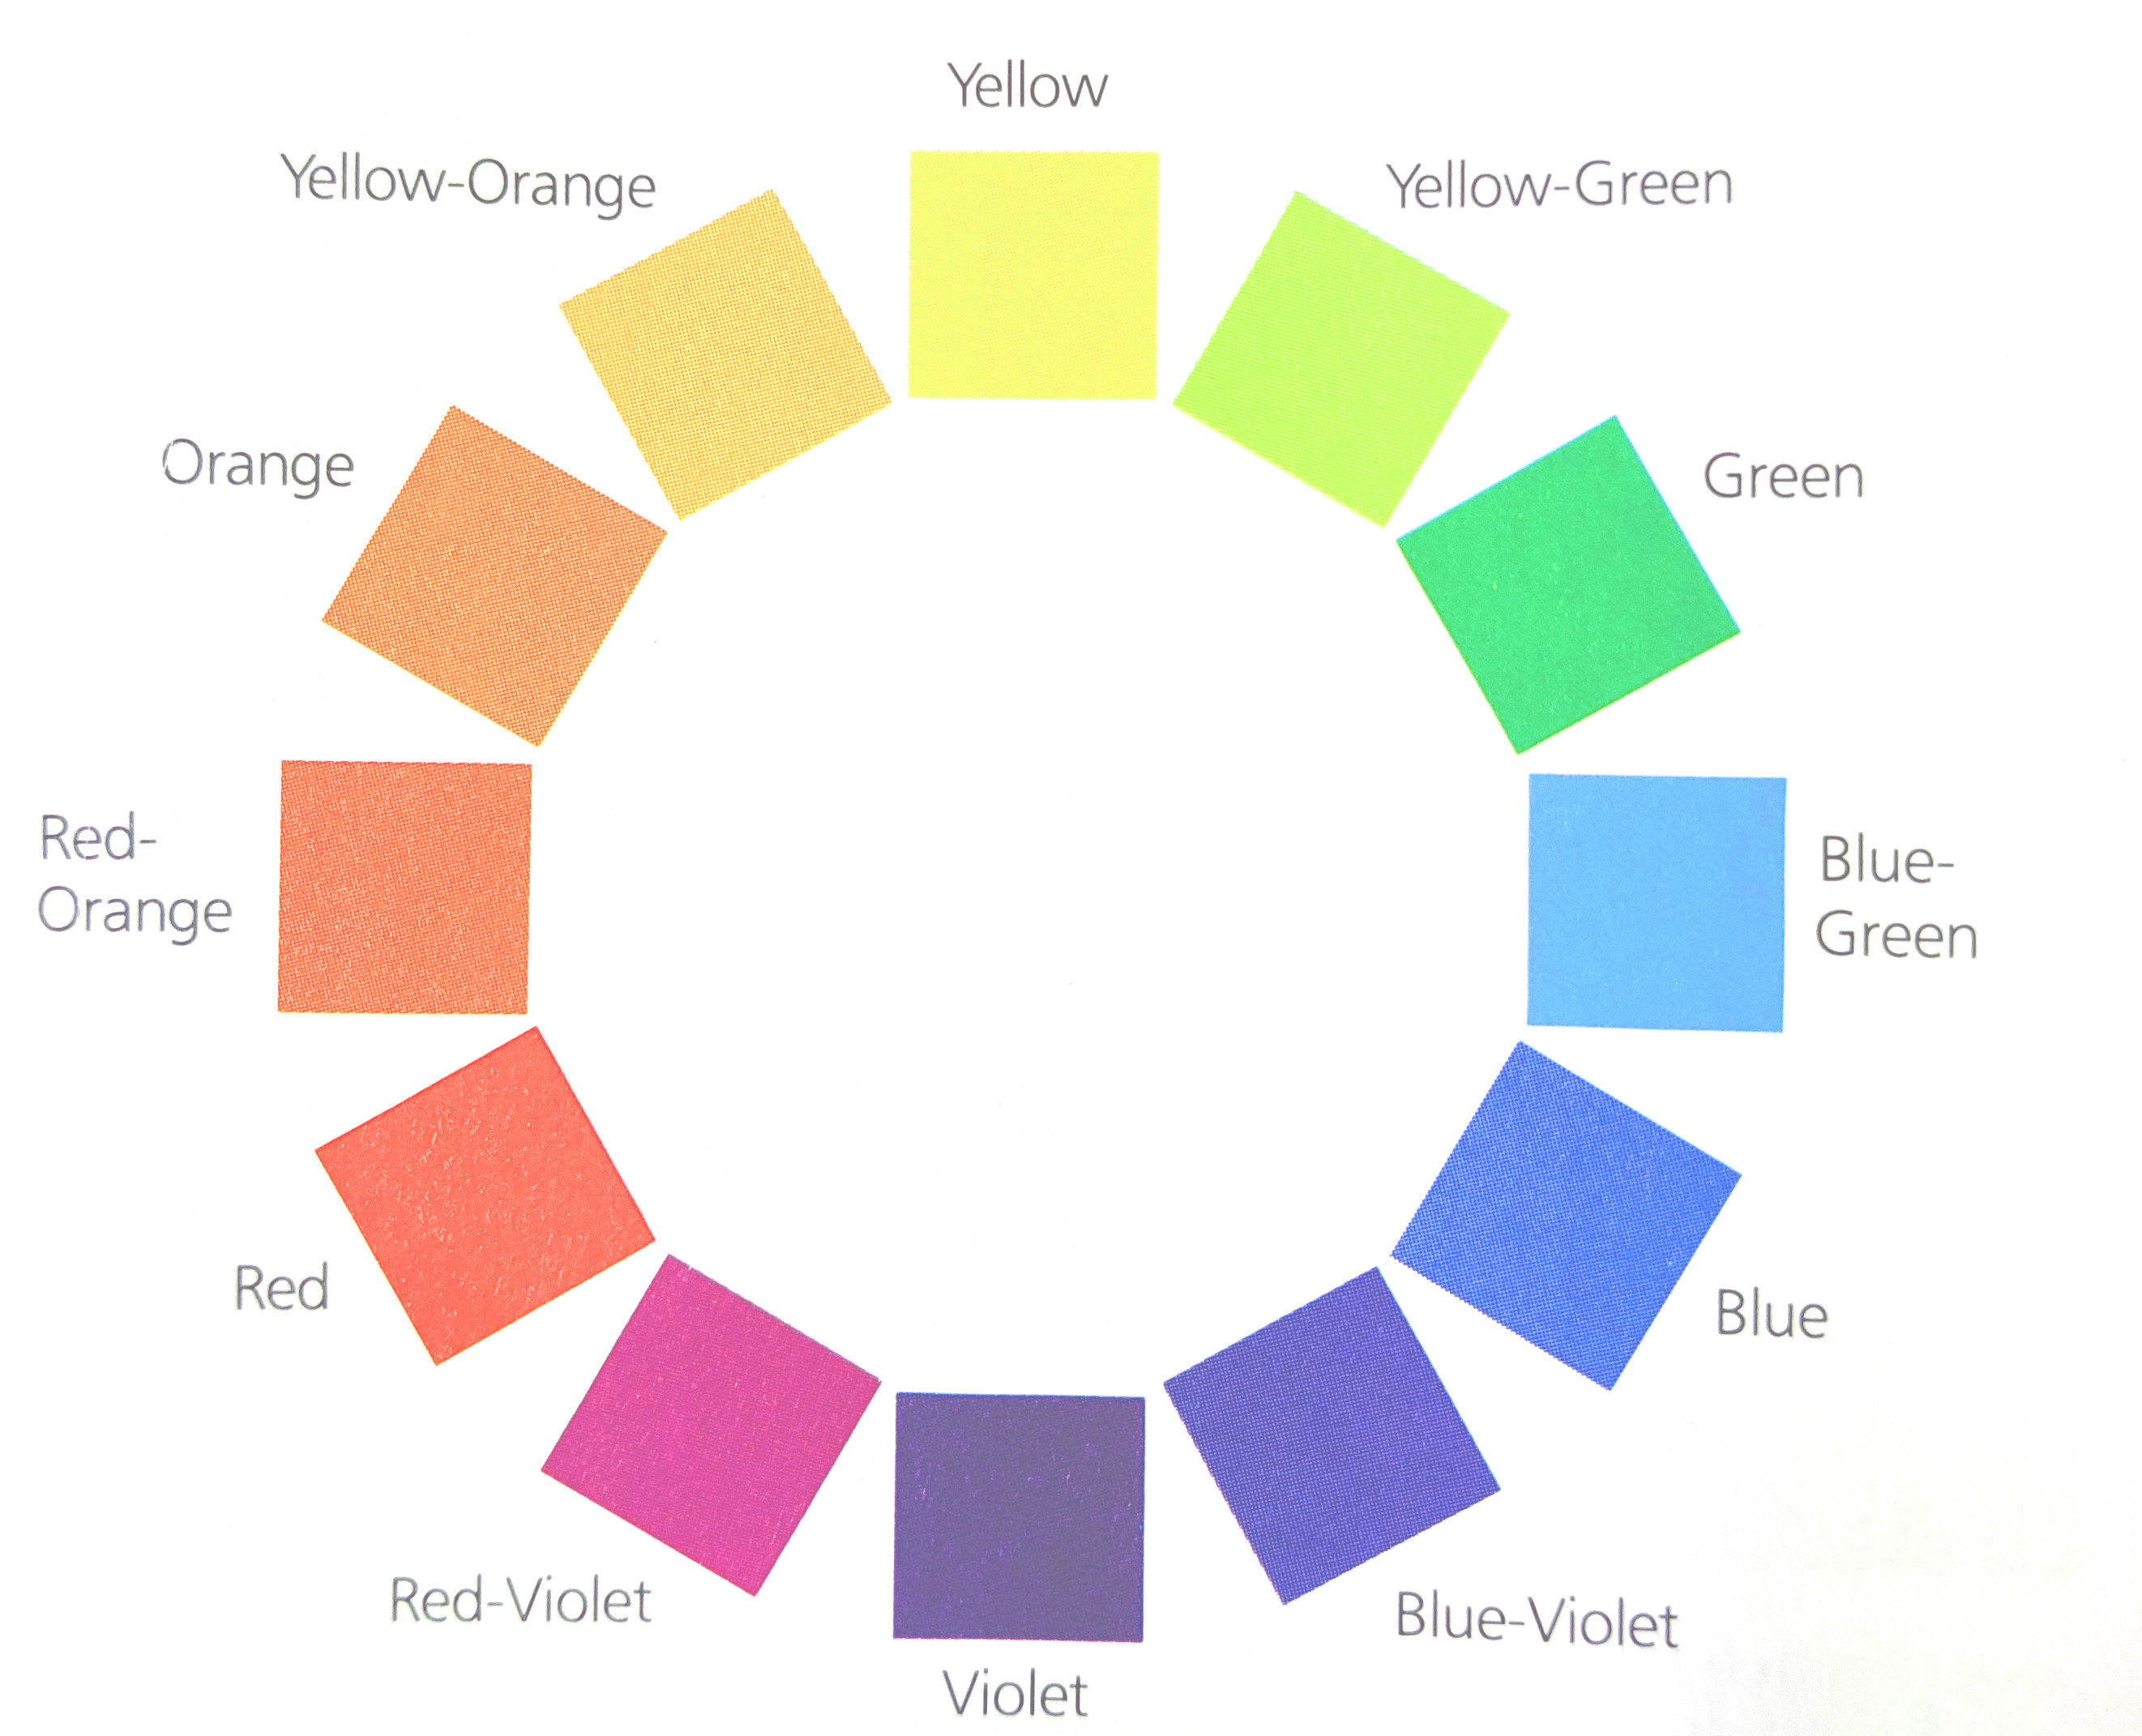
\includegraphics[width=0.2\textwidth]{figures/introduction/art aesthetics/colour_wheel.jpg}}
    \caption{Examples of Colour}
    \label{fig:colorwheel}
\end{figure}

Many formalist attributes are used in hand crafted IAQA, and a consideration to wider aesthetics is included as there may be novel applications of computer vision to art criticism. One such high-level example of formal aesthetics is shown in figure \ref{fig:elements of design}; a focused example of features in IAQA literature is shown in table \ref{tab:aes_attribs}.

\begin{figure}[h!]
    \centering
    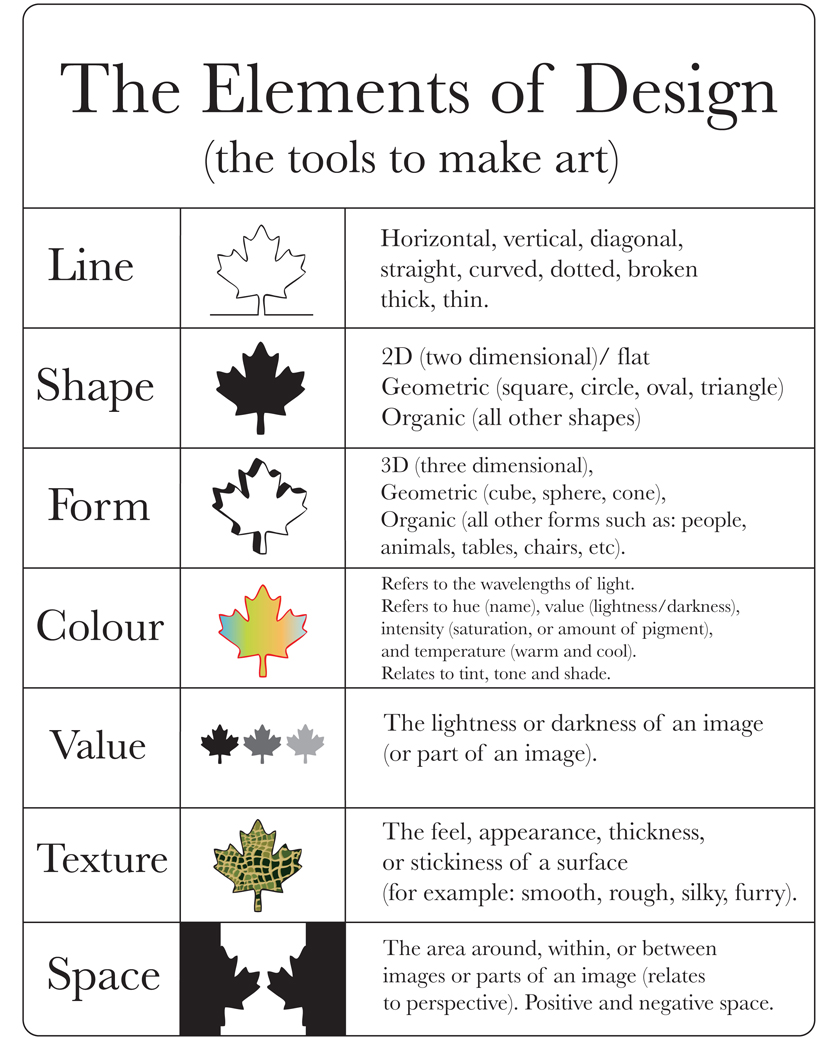
\includegraphics[height=0.4\textwidth]{figures/introduction/art aesthetics/elements3.jpg}
    \caption{Elements of Design \cite{Butler2012}}
    \label{fig:elements of design}
\end{figure}

\subsection{Photo Aesthetics}

Photographic aesthetics within the field of IAQA have focused on so-called 'formal photographic rules', which overlap with more widely applied aesthetic rules, but have distinct properties which are a result of physical properties: lens (bokeh, Depth of Field(DOF), shutter speed), sensor, and light. Within traditional handcrafted approaches, this involved high-level attributes such as \textit{simplicity, colourfulness, color combination(harmony), sharpness, image pattern, and object composition}\cite{Liu2017a,Mavridaki2015,Datta2006,Tang2013a,Simond2015,Lo2013}. These are informed by texts on photography that themselves frequently borrow from formalist art aesthetics, which have, in turn, been sources from which high-level features are defined. 

\begin{figure}[ht!]
\centering
    \subfloat[Complimentary Colors(Color Contrast) Yellow/Blue  \cite{Ke2006}]{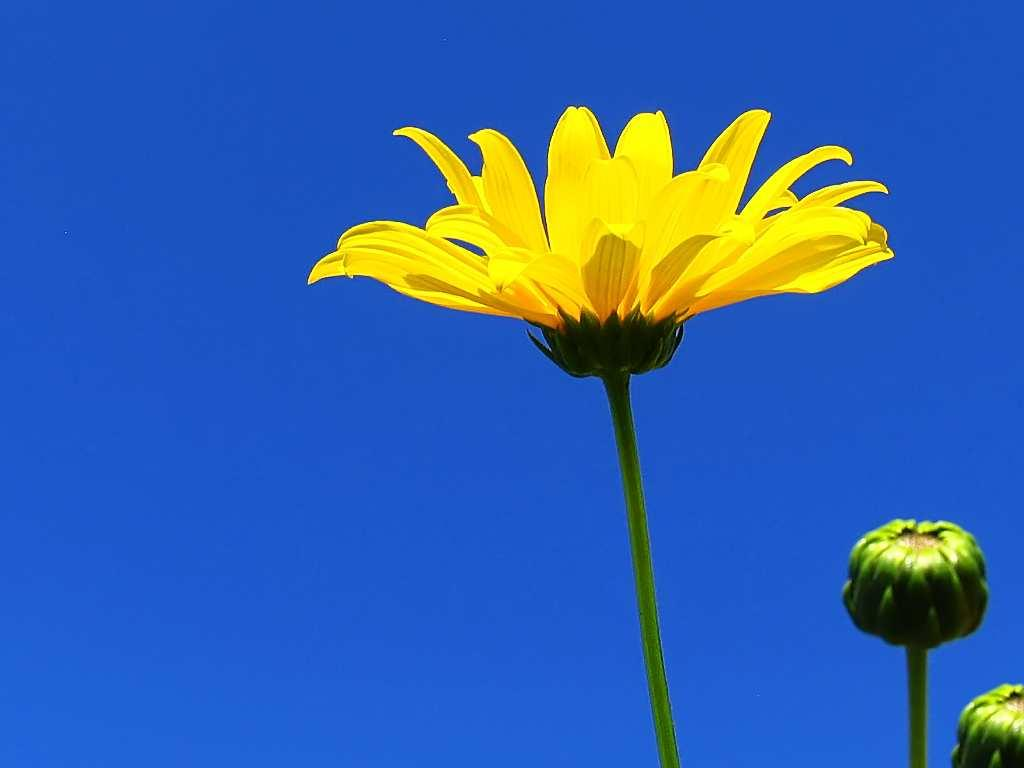
\includegraphics[width=0.2\textwidth]{figures/introduction/photo aesthetics/flower_contrast.jpg} \label{fig:colour contrast}}
    \hfill
     \subfloat[ Colour Harmony \cite{Lo2013}]{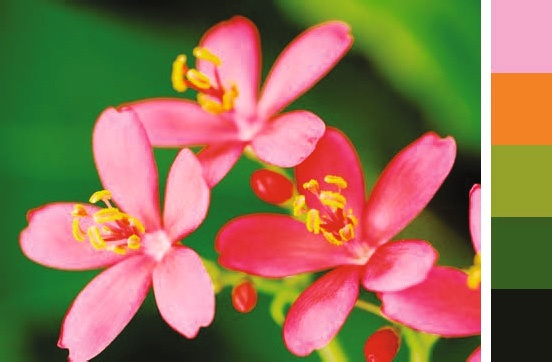
\includegraphics[width=0.2\textwidth]{figures/introduction/photo aesthetics/harmony.jpeg}
     \label{fig:harmony}}
     \hfill
     \subfloat[ Shutter Speed \cite{Lo2013}]{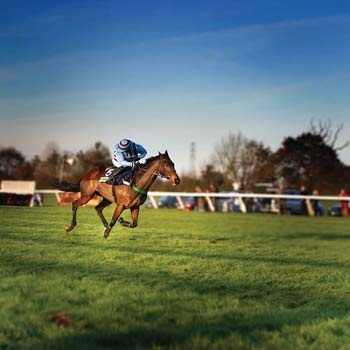
\includegraphics[height=0.15\textwidth]{figures/introduction/photo aesthetics/shutter speed.jpeg}
     \label{fig:shutter speed}}
    \vfill
    \subfloat[Rule of thirds \cite{Mai2011a}]{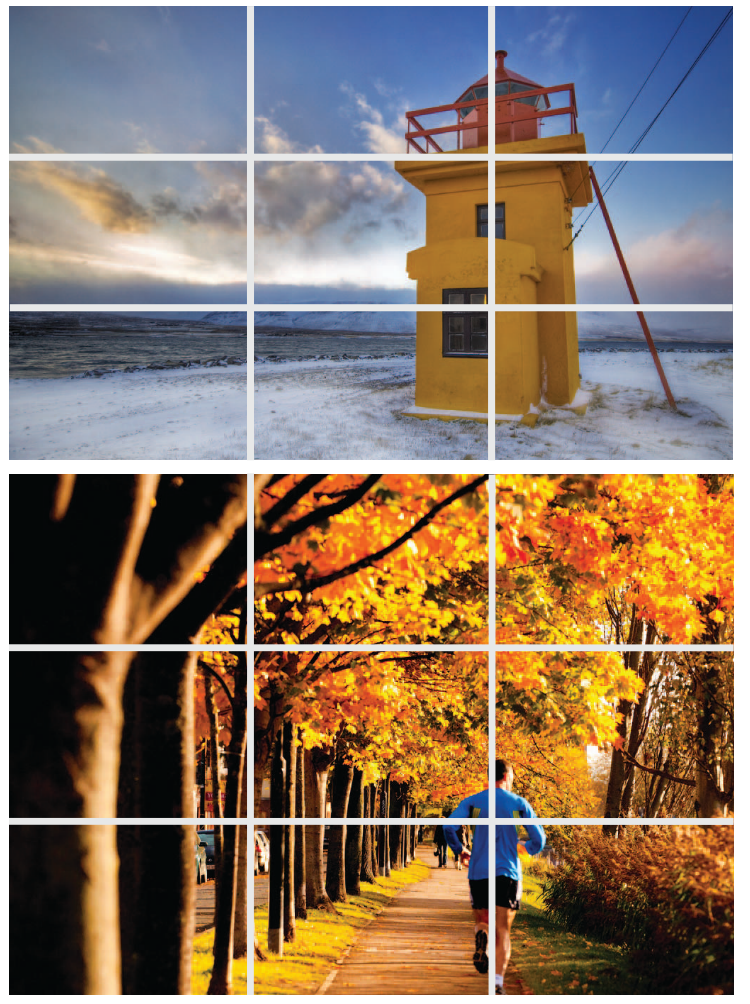
\includegraphics[height=0.2\textwidth]{figures/introduction/photo aesthetics/rule of thirds.png}
    \label{fig:composition}}
    \hfill
    \subfloat[Shallow Depth of Field (Blurring Background) \cite{Ke2006}]{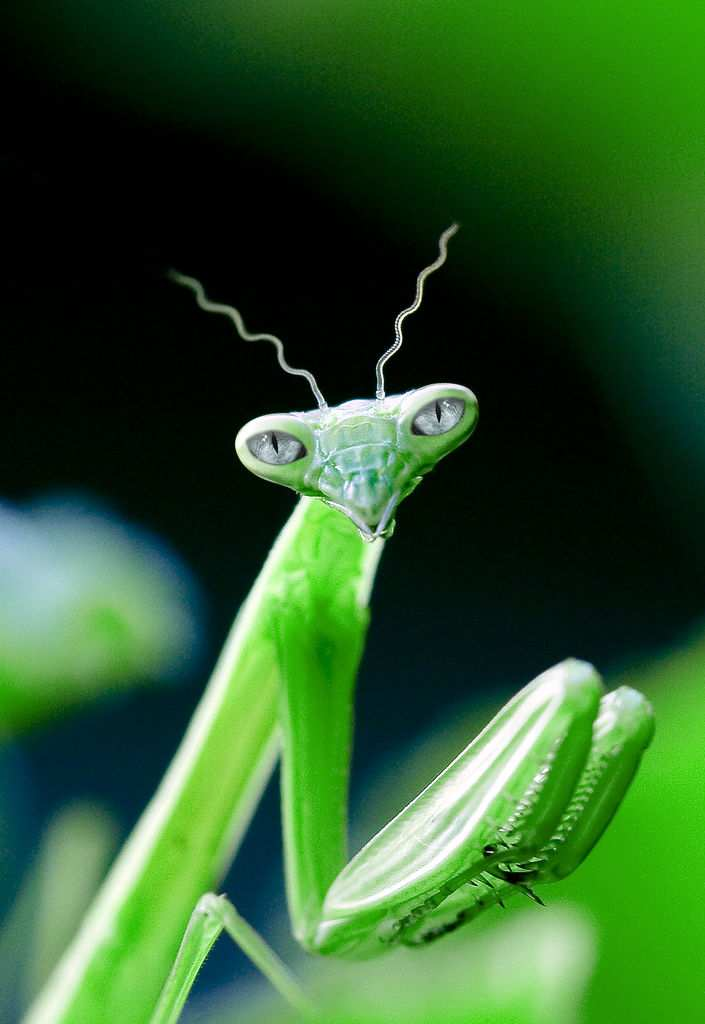
\includegraphics[height=0.2\textwidth]{figures/introduction/photo aesthetics/Look Intoby Josh Brown.png}\label{fig:object emphasis}}
    \hfill
    \subfloat[Good Lighting \cite{Lo2013}]{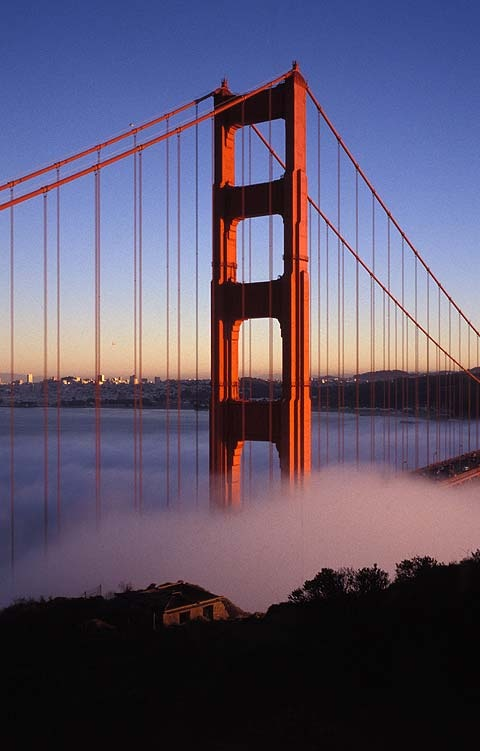
\includegraphics[height=0.2\textwidth]{figures/introduction/photo aesthetics/good_lightin.jpeg} \label{fig:lighting}}
    \caption{Examples of Photographic Formal Aesthetics}
    \label{fig:attr}

\end{figure}


Others have sought to define more abstract features, such as spatial richness\cite{Lo2013} and similarity measure\cite{Datta2006}; aesthetic attributes that are concepts of a hypothetical viewer mapped onto ranking measures. Table \ref{tab:aes_attribs} shows attributes frequently used in IAQA literature, many of which are defined within photographic texts, photo guides or researchers' own experience. It is also clear from, for instance, attributes like \textit{good lighting} are not necessarily easy to define though they may appear obvious, and that these include detailed aspects such as chiaroscuro, dynamic range, and contrast. 

\par Further, these attributes are not strictly cumulative and/or necessarily combinatorial - attributes that may constitute a \textit{good} photograph for one subject would not necessarily be effective should the subject be elsewhere. There are numerous examples of this in the datasets section of the appendix  \ref{iaqa datsets appendix}. 

\par However, it is also clear that having an intuition as a photographer is part of the aesthetic toolkit, and a re-combinatorial approach - using the right effects alongside the adjustment of camera settings, lense choice - is a part of what makes 'good photography'.

\par Figure \ref{fig:composition} bottom clearly has \textit{rhythm, colour harmony, composition} created by the object of the photograph being at the intersection of the golden ratio, the colour of the leaves, the repetition of trees and it also makes use of perspective - an image figure \ref{fig:lighting} shallow DOF(wide lens iris aperture/low $f$ number)  would be not be a useful attribute and would render the bridge out of focus. Attributes such as shallow DOF that in one context (portraiture or macro photography) are part of highlighting a salient object that in another (landscape photography) would degrade the image aesthetics quality\footnote{$f$ 64 is a renowned landscape movement which makes use of extremely small apertures-rendering almost everything in focus to create a painterly quality of image, examples of this can be seen on the Metropolitan Museum of Art's web-page:  \href{https://www.metmuseum.org/toah/hd/f64/hd_f64.htm}{https://www.metmuseum.org/toah/hd/\f64/hd\_f64.htm}}. Many of the low quality images in the qualitative examples of IAQA datasets (section \ref{iaqa datsets appendix} of the appendix) show images that might otherwise be high quality but the image has of shallow DOF with a salient object that is out of focus.

\begin{table}[t]
\centering
\small 
\begin{tabular}{p{0.2\textwidth}<{\centering}?cp{0.5\textwidth}}
\specialrule{0.1em}{0.1em}{0.1em}
 \multicolumn{3}{c}{Example Aesthetic Attributes}\\
 \specialrule{0.1em}{0.1em}{0.1em}
  \textbf{Feature(aesthetic Attribute)}  & \textbf{Figure} & \textbf{Description}\\
  \specialrule{0.1em}{0.1em}{0.1em}
  Rule of Thirds/ Object Composition & \textbf{\ref{fig:composition}} & Salient or important elements placed on lines of image divided into $3\times3$ grid. Ratio of $1.61803$ \cite{Yeh2012}\\
  
  \specialrule{0.05em}{0.1em}{0.1em}
  Saturation/ Hue Saturation &\textbf{\ref{fig:colour contrast}} & saturation indicate chromatic purity (emphasis of single color value) \cite{Datta2006} \\
  
  \specialrule{0.05em}{0.1em}{0.1em}
  Simplicity &\textbf{\ref{fig:colour contrast}} & Keeping single subject or saline object well composes and not having too many subjects in frame.\cite{Tang2013a}\\
  
  \specialrule{0.05em}{0.1em}{0.1em}
  Color Combination & \textbf{\ref{fig:harmony}} & Color Distribution of image finding a few dominant colours\cite{Lo2013,Tang2013a}\\
  
  \specialrule{0.05em}{0.1em}{0.1em}
  Lighting & \textbf{\ref{fig:lighting}} & lighting contrast between foreground and background, use of effects such contrast\cite{Kong2016, Lo2013}\\
  
  \specialrule{0.05em}{0.1em}{0.1em}
  Sharpness & \textbf{\ref{fig:object emphasis}} \ & Subject in focus, use of depth of field and lighting to isolate salient object from background\cite{Mavridaki2015a}\\
  
  \specialrule{0.05em}{0.1em}{0.1em}
  Image Pattern & \textbf{\ref{fig:composition} bottom}& Use of symmetry and texture to crate harmony and rhythm\cite{Mavridaki2015a,Kanwal2021}\\
  \specialrule{0.1em}{0.1em}{0.1em}
\end{tabular}
\caption{ Aesthetic Attributes from IAQA Literature}
\label{tab:aes_attribs}
\end{table}


One further aspect of photo aesthetics that is important to consider is the properties of the camera, this might include resolution of sensor, bit depth of color, alongside the sharpness of lens which effects both features such as chromatic aberrations (red, blue halo at object edge) and resolving power of lenses, many of these properties are interrelated. For instance small $f$ number (aperture) increase sharpness even for low quality lenses but also increase DOF. Other aspects include tilt and shift (figure \ref{fig:tilt shift all egs}) where a specialist lens or large format camera might be used in architecture photography to correct perspective. 



\newpage    
\section{Applications}


\subsection{Commercial Applications and Practical Applications}

Applications include image recommendation, photo album optimisation\cite{Liu2017} and advertising, alongside image enhancement\cite{Talebi2018} and on-device real time IAQA. Others have utilised image captioned ground truth to train models that have then been able to offer advice to photographers, providing feedback on aspects of technique and camera operation such as,\textit{`a greater depth of field of say f8 would have produced an over all better shot'}\cite{Jin2019}, these latter approaches have also made use of attributes' radar maps\cite{Jin2019}. Another related approach is 'best hand shot'\cite{Schwarz2018a} which utilises the multi-capture feature that many smart phones are now equipped with.

\begin{figure}[ht!]
    \centering
    \subfloat[Image Before Enhancement Enhancement\cite{Talebi2018}]{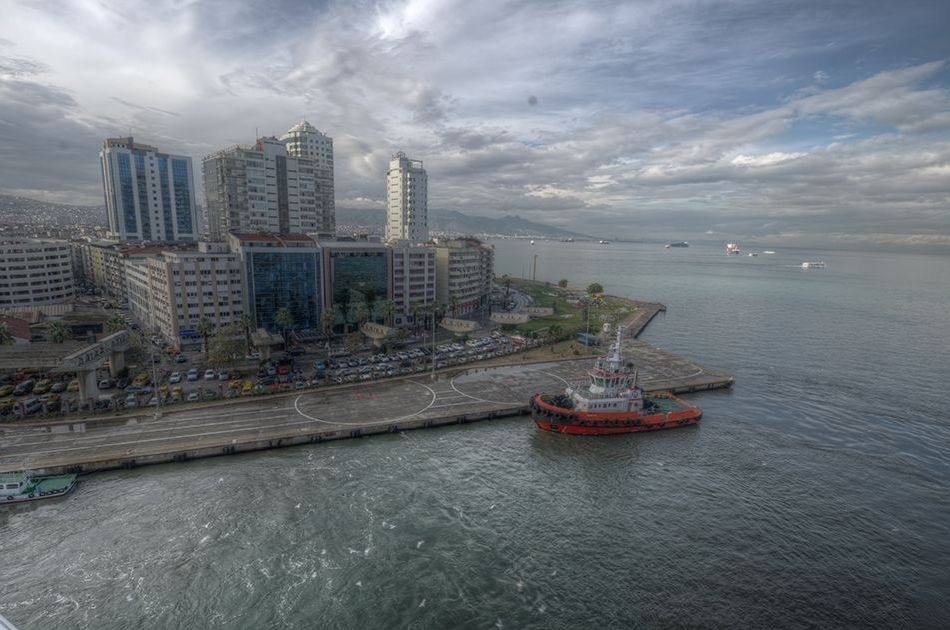
\includegraphics[width=0.2\textwidth]{figures/introduction/examples of applications/11Talebi, Milanfar - 2018 - NIMA Neural Image Assessment-annotated.pdf1.jpeg}}
    \vspace{3mm}
    \subfloat[Image Before Enhancement\cite{Aydin2015}]{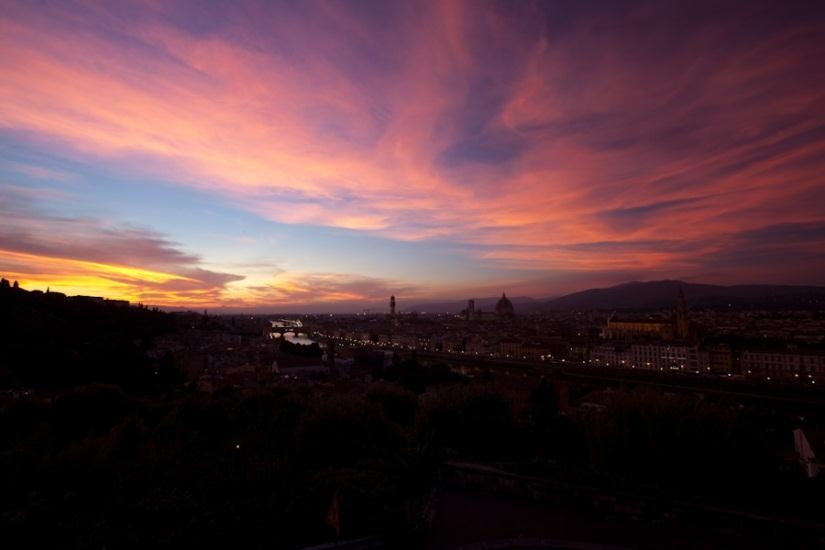
\includegraphics[width=0.2\textwidth]{figures/introduction/examples of applications/1Automated Aesthetic Analysis.pdf1.jpeg}}
    \vspace{3mm}
     \subfloat[Image Before Automatic Crop Enhancement\cite{Schifanella2015}]{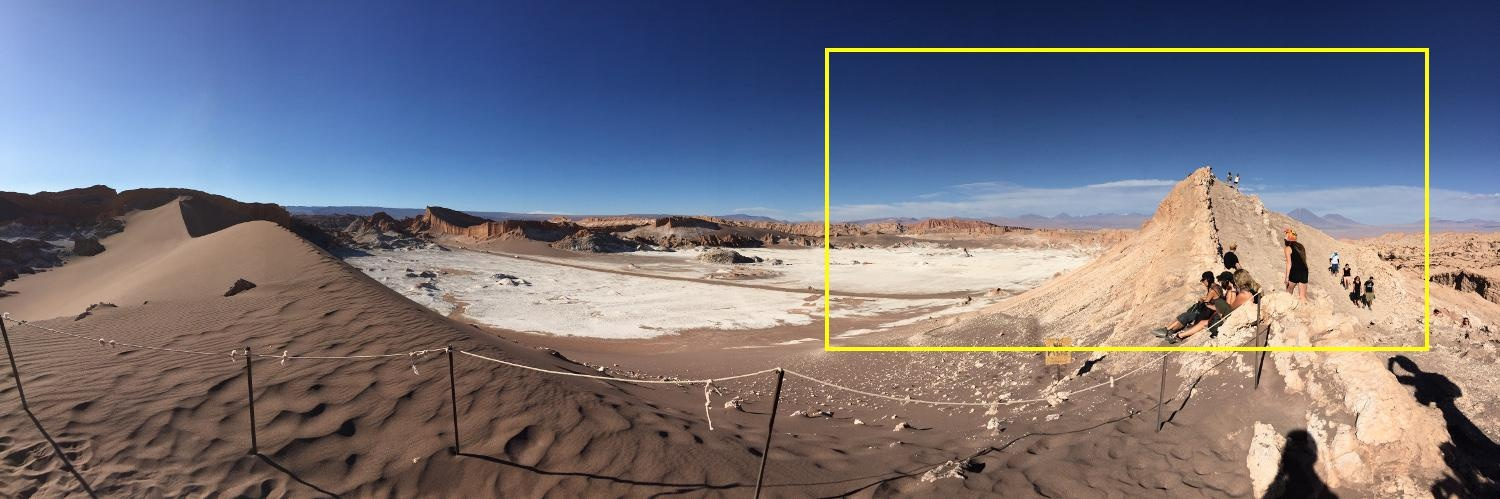
\includegraphics[width=0.2\textwidth]{figures/introduction/examples of applications/7Learning to Compose with Professional Photographs on the Web.pdf5.jpeg}}
    \vfill 
    \subfloat[Image After Enhancement Enhancement\cite{Talebi2018}]{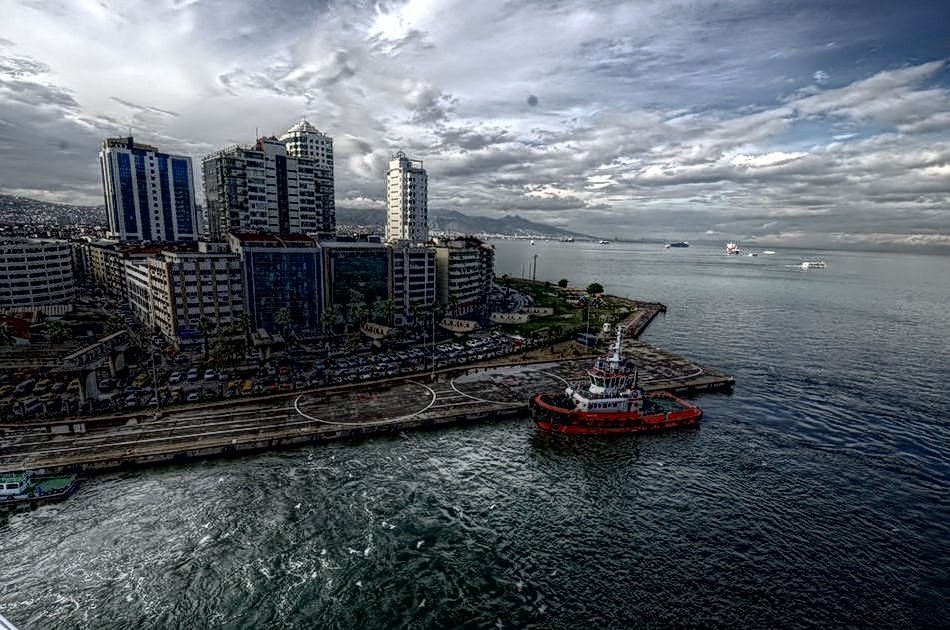
\includegraphics[width=0.2\textwidth]{figures/introduction/examples of applications/11Talebi, Milanfar - 2018 - NIMA Neural Image Assessment-annotated.pdf2.jpeg}}
    \vspace{3mm}
    \subfloat[Image After Enhancement  Enhancement\cite{Aydin2015}]{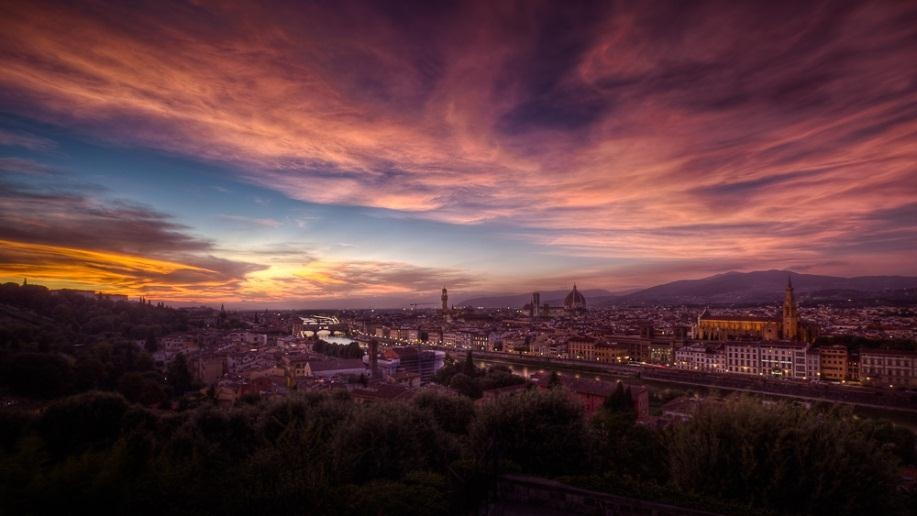
\includegraphics[width=0.2\textwidth]{figures/introduction/examples of applications/1Automated Aesthetic Analysis.pdf4.jpeg}}
    \vspace{3mm}
    \subfloat[Image After Automatic Crop Enhancement\cite{Schifanella2015}]{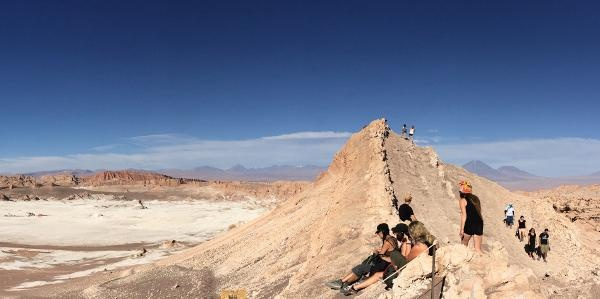
\includegraphics[width=0.2\textwidth]{figures/introduction/examples of applications/7Learning to Compose with Professional Photographs on the Web.pdf6.jpeg}}
    \caption{Image Enhancement Examples From IAQA Literature}
    \label{fig:enhancement}
\end{figure}


Other applications include the selection of product photographs that are most likely to be of higher quality and hence more attractive to consumers, or of the most appealing architectural photographs of hotels. One real-world example of this is Idealo\cite{idealo2021}, who provide a service and commercial applications of IAQA\cite{Talebi2018,Lennan2018}. 

\begin{figure}[ht!]
    \centering
    \hfill
    \subfloat[On Device Rating\cite{Lo2013}]{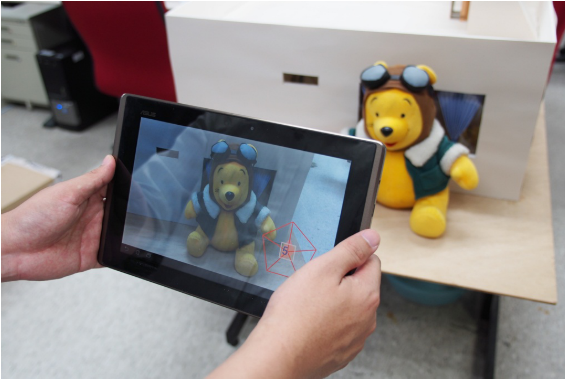
\includegraphics[width=0.2\textwidth]{figures/introduction/examples of applications/on_device.png}}
    \hfill
    \subfloat[Aesthetic Attributes\cite{Lo2013}]{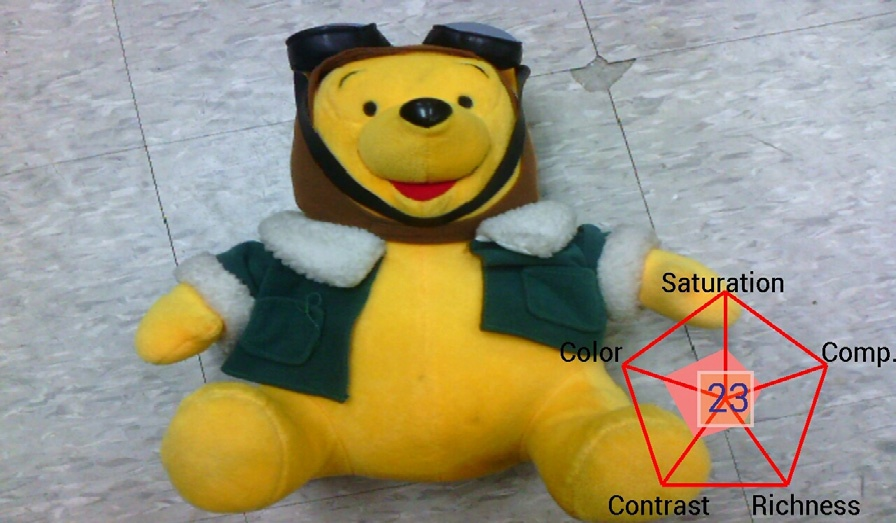
\includegraphics[width=0.2\textwidth]{figures/introduction/examples of applications/10Intelligent Photographing Interface.pdf1.jpeg}}
    \label{fig:on device}
    \hfill
    \subfloat[Predicted Attributes Scores (Radar Maps)\cite{Jin2019}]{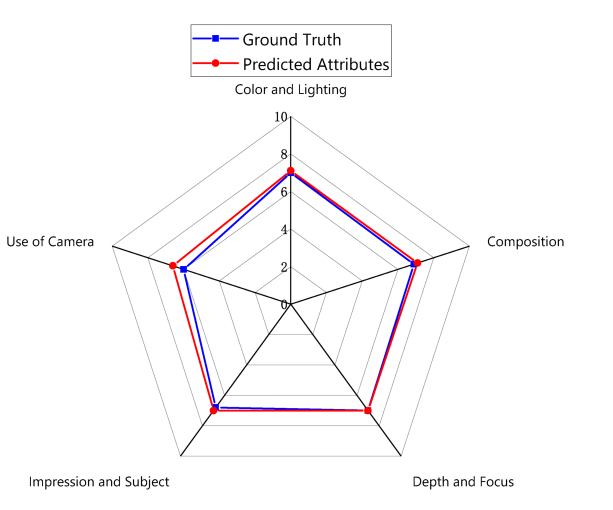
\includegraphics[width=0.2\textwidth]{figures/introduction/examples of applications/atributes_map_jin2019.png}}
    \hfill
    \subfloat[Best Handy Shot\cite{Schwarz2018a}]{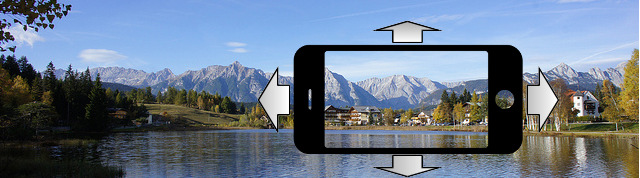
\includegraphics[width=0.2\textwidth]{figures/introduction/examples of applications/wschwarz2018a.png}}
    \caption{Application Examples (On Device Rating, and Best Hand Shot)}
    \label{fig:on device}
\end{figure}

More widely, there are numerous fascinating examples of computer vision in aesthetics - such as pose analysis of ancient art, and art restoration and verification where computer vision is being applied to verify a painting's authenticity\footnote{\href{https://art-recognition.com/}{https://art-recognition.com/}}\cite{Snow2017} and in generating novel images\footnote{\href{https://www.artbreeder.com/}{https://www.artbreeder.com/}} and include computer vision applications of style recognition\cite{Cheng2021} shown in figures (\ref{fig:origional}, \ref{fig:style}, \ref{fig:transfer}).

\begin{figure}[ht!]
    \centering
    \hfill
    \subfloat[Original Image \cite{Cheng2021}]{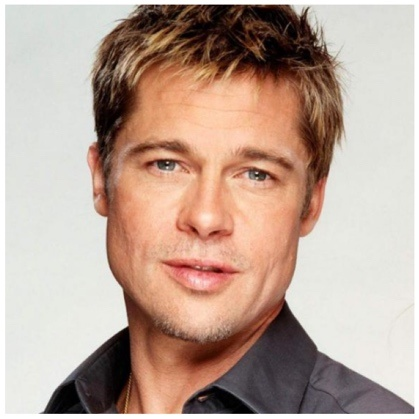
\includegraphics[width=0.2\textwidth]{figures/introduction/style_transfer_brad_pit.jpeg} \label{fig:origional}}
    \hfill
    \subfloat[Style \cite{Cheng2021}]{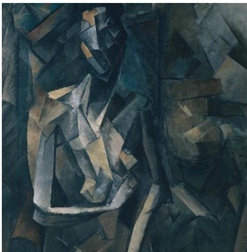
\includegraphics[width=0.2\textwidth]{figures/introduction/Syle Transfer painting.jpeg}\label{fig:style}}
    \hfill
    \subfloat[Style Transfer Image \cite{Cheng2021}]{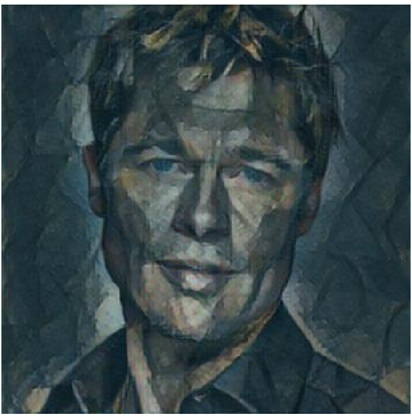
\includegraphics[width=0.2\textwidth]{figures/introduction/Arbitrary_Style_Transfer.jpeg}\label{fig:transfer}}
    \label{fig:style transfer}
    \caption{Examples of Style Transfer}
    
\end{figure}


\newpage


\section{Aesthetics: A Computer Vision Problem}

Computer vision has focused applications stenography \cite{Das2021}, texture analysis,semantic segmentation\cite{Shelhamer2017}, 3D scene reconstruction\cite{Murez2020}, super-resolution\cite{Liang2021} and edge detection\cite{Poma2021} as well as more widely in areas such as object recognition, image captioning, medical imaging. Prior to deep learning  approaches, many techniques involved extracting features using Discreet Wavelet Transoms (DWT)\cite{Makbol2013, Goel2019, Kanwal2021, Goel2014} and  handcrafted or combinations of low and high level feature extraction, where support vector machines (SVMs) are used to enhance for multi-class or object recognition\cite{Makili2011,Goos2016}. 

\par While many of these methods continue to be researched, more recent approaches use Deep Learning - such as attention based salience\cite{Zhu2020}, object detection\cite {Mutch2006, Lei2019, Peng2018}, classification \cite{Jia2020}, and multi-class or active learning\cite{Wu2020a, Joshi2010, Li2004, Gu2015}.

Aesthetics as computer vision problem is further addressed in the Methodology Chapter \ref{chap:Methodology}, and approaches outlined in the Literature Review \ref{chap:Literature_Review} might be considered to be at the intersection of empirical study in the aesthetics of digital photographs (DP), Image Processing (IP), and machine learning (ML). 

\par DP are quantized $\mathbb{R}2$ discrete time images of continuous signal data $\{a,b\} \implies \{x\in \mathbb{Z} : a \leq x \leq b\}$ where $a = 0.4\times{10^{- 4}}$ and $ b = 0.7\times {10^{- 6}}$ frequencies of the electromagnetic spectrum in continuous time in $\mathbb{R}3$ space. IP is a set of techniques used in processing digital images; Machine Learning is a wider umbrella term encompassing approaches such as Deep Learning and Reinforcement Learning (RL). Approaches to deep learning include Convolutional Neural Networks (CNNs)\cite{LeCun1989}, Generative Adversarial Network (GANs)\cite{Goodfellow2020}, Long-Short Term Memory (LSTM)\cite{Hochreiter1997a} and most recently Vision Transformers (ViTs)\cite{Yuan2021, Dosovitskiy2020}. Each field $\in \{DP, IP, ML\} $ (an illustration of this is shown by the Venn diagram in figure \ref{fig:IAQAVenn}) in turn might have further subsets, such as deep learned features as a supervised learning task on a particular subset of DP images, where one type of IP is used for as part of data augmentation. \cite{morris2004computer}.

Many of the traditional approaches to aesthetics have relied on the extraction of hand-crafted features, and are what art criticism would define as formalist aesthetics; texts on formal  photography such as \cite{Kodak1995take}, are frequently cited in computer vision research\cite{Mitarai2013, Murray2012,Talebi2018}. 

\par One clear and obvious drawback of hand-crafted feature extraction approaches, in light of findings across subdomains of aesthetics (empirical aesthetics, philosophy and art), which has been noted in many of the computer science publications\cite{Zhang2021d,Ke2006,Kolesnikov2020,Lu2015b,Birkhoff1933a,Brielmann2018,DaSilva2017,Skov2019} is the not unambiguous in definition(s) of attributes in compounded further by the potential for ambiguity within GT data. Further, although hand-crafted features have produced models that have been able to generalise, they have often been weak learners. Irrespective of recent gains made in computer vision using deep learning, which has come to dominate\cite{Zhang2021d}, it might be argued that these later approaches are better suited to this type of domain - as features are learned, and therefore do not rely on human defined categories but rather on how features that best predict ground truth (GT) labels. 



\subsection{Image Aesthetic Quality Assessment IAQA}

One conceptual challenge in defining a domain within aesthetics or vision is the question of whether aesthetic appreciation is cognitive, a property of stimulus itself, or something that can be objectively assessed as a quantitative and computational task. 

\par This ambiguity has been highlighted even in early canonical attempts at analysis of aesthetics; Kant in 1892, for instance, introduces in his critique of judgement the notion simultaneously that 'beauty is in the eye of the beholder'\cite{Zhang2019} while judging something as good - is to 'to make [...] a subjective assessment [of what] he has reason for expecting a similar delight from everyone'\cite{Kant1892kant}. The tension between these two statements being an attribute of 'aesthetic' experience\cite{Spratt2015}.
\par
Notwithstanding these inherent ambiguities which are nontrivial, IAQA \textit{has} been extensively researched and formulated as a computer vision problem. Addressing the question of where IQAQ `sits', however, is important in dealing conceptual ambiguity. The importance of clarifying IAQA is fourfold:
\begin{description}
\item[Enables]formulating a problem by understanding of what tools are appropriately leveraged from machine learning and pattern recognition;
\item[Disambiguates] IAQA within nomenclature and sub/super domains where there there is potential for cross over and conceptual confusion; 
\item[Identification] of opportunities for real world application, learning for other domains and clearly;
\item[Understanding] overall purpose and value. 
\end{description}

\newpage

\subsubsection{IAQA definition}

Here the term IAQA is used to disambiguate the field of enquiry, as a term most frequently used in literary criticism and to disambiguate from from fields such as Image Restoration or IQA.

\begin{wrapfigure}[15]{l}{0.5\textwidth}
\specialrule{0.01em}{0.2em}{0.2em}
     \begin{center}
     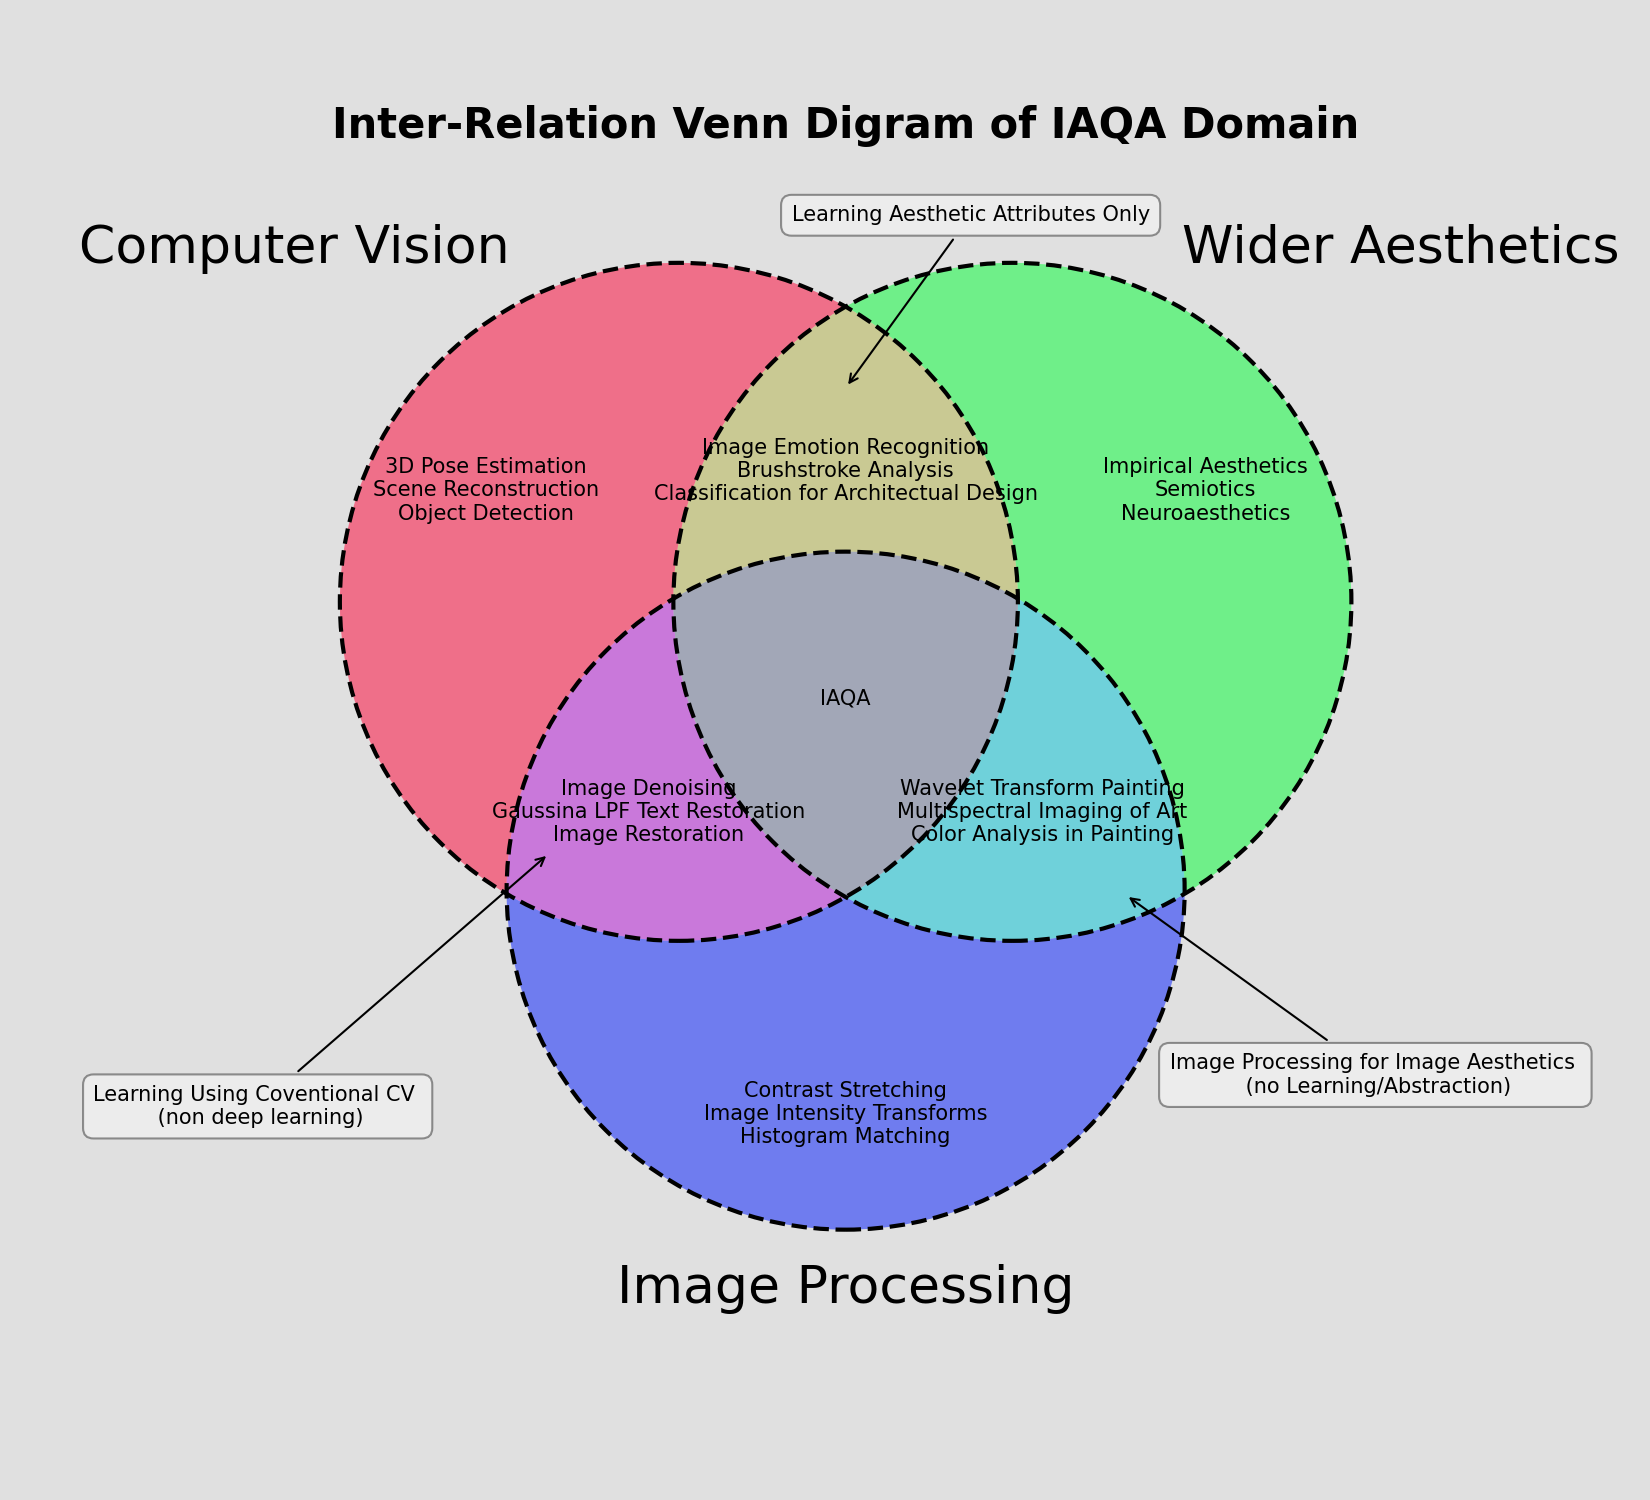
\includegraphics[width=0.45\textwidth]{figures/introduction/inter-relation_of_subjects.png}    
     \caption{Venn diagram Data sets Reviewed in literature reviews }
     \label{fig:IAQAVenn}
  \specialrule{0.01em}{0.2em}{0.2em}
  \end{center}
 \end{wrapfigure}
\par Both Image Processing and Computer Vision are included as separate fields, as there are applications for each within the wider domain of aesthetics - for example, Wavelet Entropy for painting crack identification does not necessarily constitute learning. Here, therefore, it is considered a qualifying feature if IAQA is an application of both Image Processing and Computer vision in the domain of aesthetics\cite{Constatantin2020}. 
\subsubsection{Attention Mechanisms}\\
\par
Within the domain of IAQA, there remains a significant gap between hand-crafted or deep learning models in predicting how a population of human assessors would rate  an image. Further, it is notable that the largest recent gains in predictive accuracy and ability to generalise have come from models that combine deep learning with attention mechanisms. 

\par Attention maps, for example, have been framed as optimisation models to boost a model's ability to learn, to use semantic information, identify areas of focus, or using models trained on salient object detection to inform attention patch centroids.

\subsection{Challenges for IAQA:}

Some of the technical challenges that have been demonstrated to hinder a model's ability to learn are also useful areas for domains more widely. For example image composition is a feature which is challenging to learn where input images and corresponding feature maps of a convolution neural network are necessarily square. These are inherent and no trivial examples of how a CNN might handle real world data, which is potentially messy, ambiguous, and degraded or noisy signal data.


GT is often created by a community of human participants, some of whom may be hobby photographers and others professional. It is unclear whether these rules have been rigorously followed in all cases. Further, in classification tasks or object recognition salience detection, the levels of semantic granularity applied is not so well-defined for IAQA. 

One area of complexity is the clear interplay between context and what is an aesthetic attribute of an image - for instance, a medical image may be considered aesthetically beautiful, or indeed an image from the Oxford flower dataset, and if entered into a competition may score highly. 

\par This may be, for instance, due to the subject matter having a high degree of visual interest that subjectively piques the interest of a viewer with attributes such as visual symmetry. It is clear that both image symmetry and symmetry of a salient object \textit{itself} provide both potential attributes that can be considered aesthetically high value.

\subsection{Challenges/Problem Definition}

Advances in AI in the last decade have seen super-human performance in areas such as deep reinforcement learning and domains with high dimensional search spaces, such as protein folding\cite{Senior2020} and the game of Go\cite{Silver2016}) with its $10^{170} $ possible board combinations. Digital images provide one such example of high dimensional spaces, where an 8-bit  $16 \times 16 $ Red Green Blue (RGB) channel image has $x \in \mathbb{Z} \times 2^{8^{(16 \times 16)}}$ possible pixel combinations.  

Within the wider field of computer vision, the use of deep learning techniques such as convolutional neural networks and transformers in Natural Language Processing (NLP) (and latterly, transformers for computer vision tasks) has resulted in performance accuracy that has increased year on year\cite{Sermanet2014,Simonyan2015a,Szegedy2015, He2016}. 

However, the most recent research papers published on IAQA in 2021 have not achieved accurate scores above 85\% on benchmark datasets. Many of the approaches that have improved CNNs' ability to converge faster and generalise, better such as deeper networks \cite{Simonyan2015a}, adding residual layers\cite{Krizhevsky2017a}, and improving CNN optimisation algorithms\cite{Kingma2015} have seen incremental minor improvements to IAQA.

\par
Significant improvements have generally required attention mechanisms that introduce high-level spatial inductive biases during the training of combined widening or parallel multi-column networks. Many of these represent a replacement of hand-crafted feature extraction, with crafted policies/meta heuristic inductive biases on multi column architectures. 
\par
 With recent metrics for classification CIFAR10\cite{Dosovitskiy2020} >99\% accuracy and CIFAR 100\cite{Foret2020}  96.08\%, image-net 90.88\%\cite{Dai2021}. Notably, \cite{Dai2021,Dosovitskiy2020} are both convolution transformer hybrid (ConViT) models. While \cite{Foret2020} is not a ViT-hybrid, it is only marginally better in performance than its next nearest neighbour \cite{Dosovitskiy2020}. These metrics are so accurate that it would be important to ask if an individual human subject would be able to perform so well. Many of these improvements remain within narrower applications, where CNN's have already achieved high levels of accuracy and have remained dominant\cite{Krizhevsky2017a,LeCun1998,He2016a}. 

ViTs, to our knowledge, have not been used for IAQA, have traditionally required huge datasets\cite{DAscoli2021, Touvron2020a, Khan2021}, and only generalise well on datasets (14M-300M) images\cite{Dosovitskiy2020}.

\par Datasets of this size do not exist for IAQA. Recent approaches using transfer learning are producing data efficient transformers\cite{DAscoli2021}, however it is unclear, when compared with conventional approaches on smaller tasks and on new domains, whether ViTs or ConViT's outperform CNNs. 

Here, we will \textit{compare} and \textit{contrast} the best performing CNNs with ViTs and ConViTs, and evaluate performance within the IAQA domain with binary (high, low) quality images, and attempt to predict how a compute of online voters would score an image. 

\section{Aims and Objectives}

\label{aims and objectives} 

The objective of the dissertation project outlined here is to review IAQA using the AVA benchmarking dataset as a binary classification problem. This will be outlined within the context of wider datasets and implementation challenges, and the training of state of the art models using domain adaptation vision transformers and will outline what makes IAQA important.

Key aims and objectives are:
\begin{enumerate}
    \item \textbf{Aims:} The aims of a this dissertation project are:
        \begin{itemize}
        \item To build an understanding of previous computer vision research in the domain of IAQA;
        \item To compare pre-existing CNN architectures with Vision Transformers (ViTs) and ConViTs;
        \item To further knowledge on what state of the art models can contributions in the domain of IAQA;
        \item To train, adapt and test\emph{existing models} using available code;
        \item To identify areas for future development;
        \item To generate new learning by training models that have not yet been used within IAQA such as Vision Transformers.
        \end{itemize}
    \item \textbf{Objectives:}
        \begin{itemize}
            \item To evaluate different ViT, ConViT and CNN models;
            \item To improve models by adjusting hyper perimeters and selection of appropriate data augmentation;
            \item To address challenges inherent withing the data such as \emph{class imbalance};
            \item To report metrics on architecture performance of base-line and state of the art approaches;
            \item To produce trained models that can be used for inference on unseen data;
            \item To provide provide analysis of models using both quantitative and qualitative results;
            \item To provide analysis and rational for the selection of models;
            \item To report results reproduced in by existing research withing the domain of IAQA. 
        \end{itemize}
\end{enumerate}

\section{Contributions}

The contributions made here are chiefly of a novel approach to IAQA using ViTs and ConViTs (the first application of ViTs and ConViTs) to the field of IAQA. We demonstrate this contribution by:\begin{enumerate}
\item Comparing side by side with CNNs;
\item Show both quantitative and qualitative results of inference;
\item Conducting analyse of how both transfer learning can be used with minimal additional training.
\end{enumerate}

Within literature review we conduct a review of datasets on IAQA and conduct analysis of dataset sizes and type and produce a proposed data dictionary which would be us full for further IAQA research, we also aggregate dataset size and type which is currently missing from IAQA literature and hope that this will be useful for further research within IAQA. 

We also web scrape and produce a data dictionary of all 320k images available on dpchallenge.com which would facilitate further research including multimodal research an make use of the rich comments data that is available on dp.challange.com.

We also conduct analyse of Ava Benchmark Dataset and show that their is a statistically significant relationship between the competition and mean observed score (MOS) where competition number increases monotonically with time. 

\section{Thesis Organisation}

The thesis introduction (chapter \ref{chap:Introduction}) has provided a high-level overview of the IAQA domain and potential applications. It will also introduce the current context, challenges and problems alongside providing context on aesthetics. 

\par The literature review (chapter \ref{chap:Literature_Review}) will provide context on both datasets and provide insights into how different publications have address the challenges of CV in IAQA; further it will review available data an provide justification for using the AVA Benchmark dataset based based on available literature and also outline evaluation metrics used.

\par

Research methodology (chapter \ref{chap:Methodology}) will outline the approach taken to data handling, the image processing pipeline, and to the training of models. Results and discussion (chapter \ref{chap:Results}) will provide both qualitative and qualitative outcomes of the various CNNs and ViTs that were trained. 

\par Chapter \ref{chap:Conclusion} provides future recommendations and outlines major contributions and the significance of the findings.

\newpage

\begin{enumerate}
 \item \textbf{Key Aspects:} within \ref{chap:Introduction} \emph{Introduction}.
        \begin{itemize}
            \item Introduce the application domain of IAQA \emph{aesthetics};
            \item Provide an initial outline of the problem and state of the art metrics(SoTA) on image classification;
            \item provide a \emph(lens) through which to read the following chapters. 
        \end{itemize}
 \item \textbf{Key Aspects:} within \ref{chap:Literature_Review} \emph{Literature Review}.
        \begin{itemize}
            \item A comprehensive overview of IAQA literature and analysis on different approaches taken;
            \item Evaluation of what was successful and what any drawbacks and pitfalls were within the approaches taken so far;
            \item Provide insights into how findings here can contribute to learning beyond simply attempting to supersede state of the art accuracy on the AVA benchmarking dataset. 
        \end{itemize}
    \item \textbf{Key Aspects:} within \ref{chap:Methodology} \emph{Research Methodology}.
        \begin{itemize}
        \item Vision Transformers overview and adaptation and outline models used and under what settings;
        \item Address challenges posed by the data itself such as class imbalance;
        \item Improve model performance using novel data augmentation techniques;
        \end{itemize}
    \item \textbf{Key Aspects:} within \ref{chap:Results} \emph{Results and Discussion}.
        \begin{itemize}
            \item Evaluate wider significance of research approaches including consideration of cognition and where IAQA might contribute to wider understanding within the field of computer vision;
            \item Evaluation of what was successful and what any drawbacks and pitfalls where within the approaches to IAQA thus far taken;
            \item Provide analysis and rational for selection of models used.
        \end{itemize}
     \item \textbf{Key Aspects:} within \ref{chap:Conclusion} \emph{Conclusion} .
        \begin{itemize}
            \item Explore potential future research opportunities;
            \item Outline contribution how this dissertation has contributed to existing knowledge;
            \item Identify potential novel applications, significance and importance of IAQA and computer vision research. 
        \end{itemize}
    
\end{enumerate}

The problem statement of binary classification on the AVA benchmarking dataset is outlined in the introduction and referenced, built on, and evaluated throughout the dissertation. 



